% Options for packages loaded elsewhere
\PassOptionsToPackage{unicode}{hyperref}
\PassOptionsToPackage{hyphens}{url}
%
\documentclass[
]{article}
\usepackage{lmodern}
\usepackage{amssymb,amsmath}
\usepackage{ifxetex,ifluatex}
\ifnum 0\ifxetex 1\fi\ifluatex 1\fi=0 % if pdftex
  \usepackage[T1]{fontenc}
  \usepackage[utf8]{inputenc}
  \usepackage{textcomp} % provide euro and other symbols
\else % if luatex or xetex
  \usepackage{unicode-math}
  \defaultfontfeatures{Scale=MatchLowercase}
  \defaultfontfeatures[\rmfamily]{Ligatures=TeX,Scale=1}
\fi
% Use upquote if available, for straight quotes in verbatim environments
\IfFileExists{upquote.sty}{\usepackage{upquote}}{}
\IfFileExists{microtype.sty}{% use microtype if available
  \usepackage[]{microtype}
  \UseMicrotypeSet[protrusion]{basicmath} % disable protrusion for tt fonts
}{}
\makeatletter
\@ifundefined{KOMAClassName}{% if non-KOMA class
  \IfFileExists{parskip.sty}{%
    \usepackage{parskip}
  }{% else
    \setlength{\parindent}{0pt}
    \setlength{\parskip}{6pt plus 2pt minus 1pt}}
}{% if KOMA class
  \KOMAoptions{parskip=half}}
\makeatother
\usepackage{xcolor}
\IfFileExists{xurl.sty}{\usepackage{xurl}}{} % add URL line breaks if available
\IfFileExists{bookmark.sty}{\usepackage{bookmark}}{\usepackage{hyperref}}
\hypersetup{
  pdftitle={Comparative Methods},
  pdfauthor={Brian O'Meara},
  hidelinks,
  pdfcreator={LaTeX via pandoc}}
\urlstyle{same} % disable monospaced font for URLs
\usepackage[margin=1in]{geometry}
\usepackage{color}
\usepackage{fancyvrb}
\newcommand{\VerbBar}{|}
\newcommand{\VERB}{\Verb[commandchars=\\\{\}]}
\DefineVerbatimEnvironment{Highlighting}{Verbatim}{commandchars=\\\{\}}
% Add ',fontsize=\small' for more characters per line
\usepackage{framed}
\definecolor{shadecolor}{RGB}{248,248,248}
\newenvironment{Shaded}{\begin{snugshade}}{\end{snugshade}}
\newcommand{\AlertTok}[1]{\textcolor[rgb]{0.94,0.16,0.16}{#1}}
\newcommand{\AnnotationTok}[1]{\textcolor[rgb]{0.56,0.35,0.01}{\textbf{\textit{#1}}}}
\newcommand{\AttributeTok}[1]{\textcolor[rgb]{0.77,0.63,0.00}{#1}}
\newcommand{\BaseNTok}[1]{\textcolor[rgb]{0.00,0.00,0.81}{#1}}
\newcommand{\BuiltInTok}[1]{#1}
\newcommand{\CharTok}[1]{\textcolor[rgb]{0.31,0.60,0.02}{#1}}
\newcommand{\CommentTok}[1]{\textcolor[rgb]{0.56,0.35,0.01}{\textit{#1}}}
\newcommand{\CommentVarTok}[1]{\textcolor[rgb]{0.56,0.35,0.01}{\textbf{\textit{#1}}}}
\newcommand{\ConstantTok}[1]{\textcolor[rgb]{0.00,0.00,0.00}{#1}}
\newcommand{\ControlFlowTok}[1]{\textcolor[rgb]{0.13,0.29,0.53}{\textbf{#1}}}
\newcommand{\DataTypeTok}[1]{\textcolor[rgb]{0.13,0.29,0.53}{#1}}
\newcommand{\DecValTok}[1]{\textcolor[rgb]{0.00,0.00,0.81}{#1}}
\newcommand{\DocumentationTok}[1]{\textcolor[rgb]{0.56,0.35,0.01}{\textbf{\textit{#1}}}}
\newcommand{\ErrorTok}[1]{\textcolor[rgb]{0.64,0.00,0.00}{\textbf{#1}}}
\newcommand{\ExtensionTok}[1]{#1}
\newcommand{\FloatTok}[1]{\textcolor[rgb]{0.00,0.00,0.81}{#1}}
\newcommand{\FunctionTok}[1]{\textcolor[rgb]{0.00,0.00,0.00}{#1}}
\newcommand{\ImportTok}[1]{#1}
\newcommand{\InformationTok}[1]{\textcolor[rgb]{0.56,0.35,0.01}{\textbf{\textit{#1}}}}
\newcommand{\KeywordTok}[1]{\textcolor[rgb]{0.13,0.29,0.53}{\textbf{#1}}}
\newcommand{\NormalTok}[1]{#1}
\newcommand{\OperatorTok}[1]{\textcolor[rgb]{0.81,0.36,0.00}{\textbf{#1}}}
\newcommand{\OtherTok}[1]{\textcolor[rgb]{0.56,0.35,0.01}{#1}}
\newcommand{\PreprocessorTok}[1]{\textcolor[rgb]{0.56,0.35,0.01}{\textit{#1}}}
\newcommand{\RegionMarkerTok}[1]{#1}
\newcommand{\SpecialCharTok}[1]{\textcolor[rgb]{0.00,0.00,0.00}{#1}}
\newcommand{\SpecialStringTok}[1]{\textcolor[rgb]{0.31,0.60,0.02}{#1}}
\newcommand{\StringTok}[1]{\textcolor[rgb]{0.31,0.60,0.02}{#1}}
\newcommand{\VariableTok}[1]{\textcolor[rgb]{0.00,0.00,0.00}{#1}}
\newcommand{\VerbatimStringTok}[1]{\textcolor[rgb]{0.31,0.60,0.02}{#1}}
\newcommand{\WarningTok}[1]{\textcolor[rgb]{0.56,0.35,0.01}{\textbf{\textit{#1}}}}
\usepackage{longtable,booktabs}
% Correct order of tables after \paragraph or \subparagraph
\usepackage{etoolbox}
\makeatletter
\patchcmd\longtable{\par}{\if@noskipsec\mbox{}\fi\par}{}{}
\makeatother
% Allow footnotes in longtable head/foot
\IfFileExists{footnotehyper.sty}{\usepackage{footnotehyper}}{\usepackage{footnote}}
\makesavenoteenv{longtable}
\usepackage{graphicx}
\makeatletter
\def\maxwidth{\ifdim\Gin@nat@width>\linewidth\linewidth\else\Gin@nat@width\fi}
\def\maxheight{\ifdim\Gin@nat@height>\textheight\textheight\else\Gin@nat@height\fi}
\makeatother
% Scale images if necessary, so that they will not overflow the page
% margins by default, and it is still possible to overwrite the defaults
% using explicit options in \includegraphics[width, height, ...]{}
\setkeys{Gin}{width=\maxwidth,height=\maxheight,keepaspectratio}
% Set default figure placement to htbp
\makeatletter
\def\fps@figure{htbp}
\makeatother
\setlength{\emergencystretch}{3em} % prevent overfull lines
\providecommand{\tightlist}{%
  \setlength{\itemsep}{0pt}\setlength{\parskip}{0pt}}
\setcounter{secnumdepth}{5}
\usepackage{booktabs}
\usepackage{makeidx}
\makeindex
\usepackage[]{natbib}
\bibliographystyle{plainnat}

\title{Comparative Methods}
\author{Brian O'Meara}
\date{2020-01-09}

\begin{document}
\maketitle

{
\setcounter{tocdepth}{2}
\tableofcontents
}
\hypertarget{introduction}{%
\section{Introduction}\label{introduction}}

This book was created as part of my \href{http://phylometh.info}{PhyloMeth} class, which focuses on sensibly using and developing comparative methods. It will be actively developed over the course of Spring 2017, so if you don't like this version (see date above), check back soon! The book is available \href{https://bookdown.org/bomeara/comparative-methods/}{here} but you can fork it, add issues, and look at raw source code at \url{https://github.com/bomeara/ComparativeMethodsInR}. {[}Note I'll be changing the name of the repo eventually; the course is largely in R (not entirely) but of course many key methods appear in other languages.{]}

\hypertarget{learning-objectives}{%
\subsection{Learning objectives}\label{learning-objectives}}

Readers of this book will be able to:

\begin{itemize}
\tightlist
\item
  Approach a study of a group of organisms by developing meaningful questions
\item
  Identify the appropriate methods to answer these questions
\item
  Where methods do not yet exist, be able to work on potential new methods
\item
  Understand limtations of methods and how to evaluate these limits
\item
  Draw sensible biological conclusions
\end{itemize}

\hypertarget{prerequisites}{%
\subsection{Prerequisites}\label{prerequisites}}

These are mostly prereqs for doing exercises associated with the class, but will help readers of the book, too.

\hypertarget{r}{%
\subsubsection{R}\label{r}}

Many methods are now implemented in R \citep{R-base}: the \href{http://cran.r-project.org/web/views/Phylogenetics.html}{phylogenetics task view} has a brief overview. You can also install the relevant packages that are on CRAN and R-Forge using the task view itself:

\begin{verbatim}
install.packages("ctv")
library(ctv)
install.views("Phylogenetics")
\end{verbatim}

Note that this will not install packages that are on GitHub or authors' individual websites. The \texttt{devtools} package can be useful for installing packages directly from GitHub.

\hypertarget{docker}{%
\subsubsection{Docker}\label{docker}}

Another option for installing things is to use the \href{https://hub.docker.com/r/bomeara/phydocker/}{phydocker} instance for Docker. \href{https://www.docker.com}{Docker} is (oversimplifying) like a very lightweight virtual machine. Note that it runs on Macs, Linux, Windows (Pro, Enterprise, and Education versions; for other versions, use \href{https://docs.docker.com/toolbox/toolbox_install_windows/}{Docker Toolbox}), and various cloud service providers (i.e., you could throw money at Amazon to run this on one of their servers). This instance runs a copy of RStudio Server that has most of the relevant phylogenetic packages already installed. Once you have Docker installed, you can do

\texttt{docker\ run\ -it\ -p\ 8787:8787\ bomeara/phydocker}

to run it as an RStudio Server.

If you want to use a local folder, you can use

\texttt{docker\ run\ -it\ -v\ /Path/To/My/Folder:/data\ -p\ 8787:8787\ bomeara/phydocker}

Change \texttt{/Path/To/My/Folder} to the absolute path to the folder you want access to (any subfolders will also be accessible). You can read and write to this in RStudio as the \texttt{/data} directory. In your web browser, go to \texttt{localhost:8787}, enter username and password (both are \texttt{rstudio}), to launch a version of RStudio that will run in your browser and have everything you might need. You might want to do \texttt{setwd("/data")} to make sure you're in the right directory. You can save any results or figures to this directory and it will still exist when you quit this instance.

\hypertarget{other}{%
\subsubsection{Other}\label{other}}

RevBayes, BEAST, RAxML, and much other key software implement important methods in phylogenetics but are not in R. Readers will need to install these and many more, but fortunately the authors of much of this software have excellent tutorials already.

\hypertarget{first-steps}{%
\section{First steps}\label{first-steps}}

First, understand the question you want to answer. There are a wide variety of methods, and they wax and wane in popularity, but the key to doing good science is addressing compelling questions, not using the latest method. Once you have that question, find the appropriate methods (and, depending on how early it is in the study design, the right taxa and data) to address it. Understand how those methods work, including the various ways they can fail (as all can).

\hypertarget{questions}{%
\subsection{Questions}\label{questions}}

``The currency of science is papers.''

``You need to get grants to get a job and tenure.''

Both true (for those pursuing traditional academic careers), but it can be easy to lose sight of the reason we do science: to learn about the natural world. Too often, I see students and other colleagues focus on fast ways to get high profile papers out without caring much about the questions. Some of this takes the form of what I call \protect\hyperlink{dull-model-testing}{dull model testing}: seeking to reject a trivial null that no one believed in anyway (Has diversification rate ever changed through time? Do terrestrial and aquatic species have exactly the same body size over time?). However, it can also be, ``I need to add something interesting to this basic phylogeny paper to get it published -- what can I map on the tree?'' There can also be questions asked where it seems, upon reflection, that results will not be credible (can one really estimate 999 independent diversification rates from a single tree with 500 species?).

A better approach, and one adopted in this book, is to start from questions that we actually learn something from answering. For example, we believe that how flowering plants reproduce (selfing versus outcrossing) can affect diversification rate. The first step is to ask if that is really true and show it statistically, but that is largely going to be a question of power: no one would really think that these two life history strategies would lead to exactly the same speciation rates \emph{and} exactly the same extinction rates: selfers might more readily speciate since they can settle new areas and not lack for mates, for example. One could publish a paper on just this using one of variety of methods (see \protect\hyperlink{diversification}{Diversification}) and be done. However, that is a largely sterile question: are two different things unequal? A more important question, once a difference is shown, is what this explains about the world. For example, Igic and Goldberg wondered why selfing persisted despite having a lower overall diversification rate than outcrossing. In answering that more interesting question, they found that it stemmed from subsidizing: outcrossers diversified more quickly, but transitions from outcrossing to selfing occurred much more frequently than the reverse: species moved into selfing from outcrossing, but had an overall negative diversification rate. This suggests an interesting conflict between microevolution (factors leading to selfing, in this case), and macroevolution (the differential diversification of species). In another paper, we looked at floral morphological traits to see which combinations led to higher rates of diversification (O'Meara, Smith, et al); we found one combination had a major impact, but also discovered that it was still fairly infrequent in flowering plants due to the estimated tens of millions of years required to assemble this combination from the angiosperm ancestral state. We thus learned about how slow trait evolution can hold back diversification over a very long time period.

Many interesting questions hinge on parameter estimation. How much worse is it long term to be a selfer? How long will it take to evolve multiple floral traits? How do species typically move from one habitat to another?

\hypertarget{other-resources}{%
\subsubsection{Other resources}\label{other-resources}}

There are many books and articles written about phylogenetic analysis. Some of the key books for readers of this one:

\begin{itemize}
\tightlist
\item
  \emph{Tree Thinking} \citep{BaumTreethinkingintroduction2013}
\item
  \emph{Inferring Phylogenies} \citep{felsenstein_inferring_2004}
\item
  \emph{Computational Molecular Evolution} \citep{YangComputationalmolecularevolution2006}
\item
  \emph{Phylogenetics} \citep{SemplePhylogenetics2003}
\item
  \emph{Analysis of Phylogenetics and Evolution with R} \citep{ParadisAnalysisPhylogeneticsEvolution2011}
\end{itemize}

As well as a recent \href{https://lukejharmon.github.io/pcm/chapters/}{book by Luke Harmon}.

\hypertarget{getting-data-and-trees-into-r}{%
\section{Getting data and trees into R}\label{getting-data-and-trees-into-r}}

\hypertarget{data-and-tree-object-types}{%
\subsection{Data and tree object types}\label{data-and-tree-object-types}}

In R, there are many kinds of objects. These kinds are called ``classes''. For example, take the text string ``Darwin''.

\begin{Shaded}
\begin{Highlighting}[]
\KeywordTok{class}\NormalTok{(}\StringTok{"Darwin"}\NormalTok{)}
\end{Highlighting}
\end{Shaded}

\begin{verbatim}
## [1] "character"
\end{verbatim}

It is a \texttt{character} class. \texttt{pi} is a defined constant in R:

\begin{Shaded}
\begin{Highlighting}[]
\KeywordTok{print}\NormalTok{(pi)}
\end{Highlighting}
\end{Shaded}

\begin{verbatim}
## [1] 3.141593
\end{verbatim}

\begin{Shaded}
\begin{Highlighting}[]
\KeywordTok{class}\NormalTok{(pi)}
\end{Highlighting}
\end{Shaded}

\begin{verbatim}
## [1] "numeric"
\end{verbatim}

Its class is \texttt{numeric} {[}and note that its value is stored with more precision than is printed on screen{]}.

Objects can sometimes be converted from one class to another, often using an \texttt{as.*} function:

\begin{Shaded}
\begin{Highlighting}[]
\NormalTok{example}\FloatTok{.1}\NormalTok{ <{-}}\StringTok{ "6"}
\KeywordTok{print}\NormalTok{(example}\FloatTok{.1}\NormalTok{)}
\end{Highlighting}
\end{Shaded}

\begin{verbatim}
## [1] "6"
\end{verbatim}

\begin{Shaded}
\begin{Highlighting}[]
\KeywordTok{class}\NormalTok{(example}\FloatTok{.1}\NormalTok{)}
\end{Highlighting}
\end{Shaded}

\begin{verbatim}
## [1] "character"
\end{verbatim}

\begin{Shaded}
\begin{Highlighting}[]
\NormalTok{example}\FloatTok{.2}\NormalTok{ <{-}}\StringTok{ }\KeywordTok{as.numeric}\NormalTok{(example}\FloatTok{.1}\NormalTok{)}
\KeywordTok{print}\NormalTok{(example}\FloatTok{.2}\NormalTok{)}
\end{Highlighting}
\end{Shaded}

\begin{verbatim}
## [1] 6
\end{verbatim}

\begin{Shaded}
\begin{Highlighting}[]
\KeywordTok{class}\NormalTok{(example}\FloatTok{.2}\NormalTok{)}
\end{Highlighting}
\end{Shaded}

\begin{verbatim}
## [1] "numeric"
\end{verbatim}

\begin{Shaded}
\begin{Highlighting}[]
\NormalTok{example}\FloatTok{.2} \OperatorTok{*}\StringTok{ }\DecValTok{7}
\end{Highlighting}
\end{Shaded}

\begin{verbatim}
## [1] 42
\end{verbatim}

Trying to multiply example.1 by seven results in an error: you are trying to multiply a character string by a number, and R does not automatically convert classes. Classes have many uses in R; for example, one can write a different \texttt{plot()} function for each class, so that a tree is plotted one way, while a result from a regression model is plotted a different way, but users just have to call \texttt{plot()} on each and R knows what to do.

In phylogenetics, we mostly care about classes for trees, for data, and for things to hold trees and data.

\hypertarget{tree-classes}{%
\subsubsection{Tree classes}\label{tree-classes}}

The main tree class in R is \texttt{phylo} and is defined in the \texttt{ape} package. Let's look at one in the wild:

\begin{Shaded}
\begin{Highlighting}[]
\KeywordTok{library}\NormalTok{(ape)}
\NormalTok{phy <{-}}\StringTok{ }\NormalTok{ape}\OperatorTok{::}\KeywordTok{rcoal}\NormalTok{(}\DecValTok{5}\NormalTok{) }\CommentTok{\#to make a random five taxon tree}
\KeywordTok{print}\NormalTok{(phy)}
\end{Highlighting}
\end{Shaded}

\begin{verbatim}
## 
## Phylogenetic tree with 5 tips and 4 internal nodes.
## 
## Tip labels:
## [1] "t2" "t3" "t5" "t1" "t4"
## 
## Rooted; includes branch lengths.
\end{verbatim}

\begin{Shaded}
\begin{Highlighting}[]
\KeywordTok{str}\NormalTok{(phy)}
\end{Highlighting}
\end{Shaded}

\begin{verbatim}
## List of 4
##  $ edge       : int [1:8, 1:2] 6 8 9 9 8 6 7 7 8 9 ...
##  $ edge.length: num [1:8] 1.6235 0.1432 0.0806 0.0806 0.2238 ...
##  $ tip.label  : chr [1:5] "t2" "t3" "t5" "t1" ...
##  $ Nnode      : int 4
##  - attr(*, "class")= chr "phylo"
##  - attr(*, "order")= chr "cladewise"
\end{verbatim}

This is the one used in most packages. However, it has some technical disadvantages (sensitivity to internal structure, no checking of objects) that has led to the \texttt{phylo4} format for trees and \texttt{phylo4d} for trees plus data in the \texttt{phylobase} package. Other packages add on to the \texttt{phylobase} format (i.e., \texttt{phytool}'s \texttt{simmap} format) but these are typically not shared across packages.

\hypertarget{sequence-data}{%
\subsection{Sequence data}\label{sequence-data}}

The \href{https://www.bioconductor.org/}{BioConductor} community has put a lot of effort into making R work with high throughput data, though python is still likely more popular (just remember that python 3.x is the only currently supported version -- python 2.x should not be used any longer). The \href{http://seqinr.r-forge.r-project.org/}{seqinr} package has some useful functionality for handling sequences. \href{https://www.rdocumentation.org/packages/ape/}{ape} and \href{https://github.com/KlausVigo/phangorn}{phangorn} have functions for handling data, including reading FASTA and NEXUS files in ape.

\hypertarget{other-character-data}{%
\subsection{Other character data}\label{other-character-data}}

This can include data such as discrete traits (has wings / wingless), continuous traits (body mass), geographic traits (latitudes and longitudes, which continents they occur on), and many more. These are typically loaded either as csv files from some other source or directly from an R package. This is a rapidly developing field, but many of the most useful packages are supported by \href{https://ropensci.org/packages/}{rOpenSci} -- there are packages for getting information from GBIF, eBIRD, iNaturalist, NCBI, and many more sources.

\hypertarget{phylogenies}{%
\subsection{Phylogenies}\label{phylogenies}}

The most common way to load trees is to use \texttt{ape}'s functions:

\begin{verbatim}
phy <- ape::read.tree(file='treefile.phy')
\end{verbatim}

To get a tree in \href{http://evolution.genetics.washington.edu/phylip/newicktree.html}{Newick format} (sometimes called Phylip format): essentially a series of parenthetical statements. An example (from \texttt{ape}'s documentation) is \texttt{((Strix\_aluco:4.2,Asio\_otus:4.2):3.1,Athene\_noctua:7.3);}. The format name comes from the name of the \href{http://newicks.com}{lobster house} where several major phylogenetic software developers met to agree on a tree format.

You can use the same function to enter tree strings directly, changing the argument from the \texttt{file} containing the tree to \texttt{text} containing the tree string:

\begin{Shaded}
\begin{Highlighting}[]
\NormalTok{phy <{-}}\StringTok{ }\NormalTok{ape}\OperatorTok{::}\KeywordTok{read.tree}\NormalTok{(}\DataTypeTok{text =} \StringTok{\textquotesingle{}((Strix\_aluco:4.2,Asio\_otus:4.2):3.1,Athene\_noctua:7.3);\textquotesingle{}}\NormalTok{)}
\end{Highlighting}
\end{Shaded}

Note the trailing semicolon.

One thing that can trip users up with \texttt{read.tree()} (and the \texttt{read.nexus()} function, below) is that the output class depends on the input. If you read from a file with one tree, the returned output is a single tree object with class \texttt{phylo}. You can then use \texttt{plot()} on this object to draw the tree, pass this object into a comparative methods package to estimate rates, and so forth. If the file has more than one tree, the returned class is \texttt{multiphylo}: \texttt{plot()} will automatically cycle through plots as you type return, most comparative method implementations will fail (they are written to expect one tree of class \texttt{phylo}, not a vector of trees in a different class). \texttt{read.tree()} has an optional \texttt{keep.multi} function: if set to TRUE, the class is always \texttt{multiphylo}, and you can always get the first tree by getting the first element in the returned object:

\begin{verbatim}
phy.multi <- ape::read.tree(file='treefile.phy', keep.multi = TRUE)
phy <- phy.multi[[1]]
\end{verbatim}

For NEXUS formatted files (Maddison et al., 2007), \texttt{ape}'s \texttt{read.nexus()} function can pull in the trees (and its \texttt{read.nexus.data()} function can pull in data from a NEXUS file). NEXUS is a very flexible format, and there are valid NEXUS files that still cause errors with \texttt{ape}'s function. A more robust function to read in NEXUS trees is the package \texttt{phylobase}'s \texttt{readNexus()} function (note the lack of a period and different capitalization of Nexus from \texttt{ape}'s similar function). \texttt{phylobase} uses a different structure to store trees than \texttt{ape} does.

\href{https://github.com/YuLab-SMU/tidytree}{tidytree} is still fairly new, but it is a popular way for dealing with trees for those who have been converted to the \href{https://www.tidyverse.org/}{tidyverse}.

\hypertarget{great-scientists-steal}{%
\subsubsection{Great scientists steal}\label{great-scientists-steal}}

Scientists have been creating trait-based phylogenetic trees for decades. These scientists are often experts in their group, in potential problems in their data, in how to use relevant software. In other words, their trees are likely to be better than any you make. Traditionally, these trees are published as a figure in a paper, largely unavailable for reuse. This hurts reproducibility, makes it less likely for the work to be cited, and stymies scientific progress in general. However, the field is increasingly moving to more frequent deposition of trees in reusable form: sometimes based on author initiative, sometimes based on journal requirements. The main repository for this is \href{http://treebase.org}{TreeBase}: if you are reading a paper, and want to use its tree, that's the first place to look. You can also use their website to search for taxa. The trees can be downloaded and loaded into R using \texttt{phylobase} (the NEXUS format used by TreeBase is hard for \texttt{ape} to load).

Another approach that is growing in importance is \href{http://otol.org}{Open Tree of Life}. It seeks to synthesize thousands of trees to create a single tree of life. The \texttt{rotl} package can download this synthetic tree or components of it (the tree for a particular genus, for example). For most groups, however, the synthetic tree is largely based on taxonomy, so it is not very resolved. This is improving as the database of trees available for Open Tree's synthesis grows (to add to it, go to \_\_\_\_\_\_\_\_\_\_\_\_\_\_\_\_\_\_\_), but for most scientific studies, I wouldn't currently suggest using the synthetic tree (but for getting a sense for a group, making a tree for a class, it can be useful; also see the \href{http://www.phylotastic.org}{Phylotastic} project for ways to use trees in teaching or other purposes). However, the Open Tree project also has a cache of thousands of trees that have been hand curated (taxonomic names resolved, ingroups specified, tree type recorded, etc.). The \texttt{rotl} package lets you download these, too. For most analyses, you want trees with branch lengths, and so you can download just chronograms. For example,

\begin{Shaded}
\begin{Highlighting}[]
\CommentTok{\#rotl::\_\_\_\_\_\_\_\_\_\_\_\_\_\_\_\_\_}
\end{Highlighting}
\end{Shaded}

Two important notes about reusing trees:

\begin{itemize}
\tightlist
\item
  \textbf{Give credit}: If your entire paper is based on the tree from one other paper, you \textbf{must} cite that paper (and also the ways you got the tree, including the packages and/or repositories). If it's based on trees from around a dozen papers, you should cite them, too. If you're getting into the hundreds, many editors will object to properly citing them all, but one compromise approach until a better way of giving credit appears is to have supplemental info or an appendix with citations for all the relevant papers (including DOIs to make these easier to parse later)
\item
  \textbf{Tree quality matters}: As you will see in later sections, many comparative methods are based on using branch lengths: look at different rates of character evolution, looking at diversification rates over time, etc. If your starting tree is wrong, even if the topology is perfect but the branch lengths are wrong, later downstream analyses are also likely to be wrong. Some methods (like independent contrasts) are fairly robust to this (\_\_\_\_\_\_\_\_\_\_\_\_\_\_\_\_\_\_), but the field has not tested many others yet, and most should be far more sensitive than contrasts. This matters less if you are testing dull hypotheses (see Chapter \_\_\_\_\_\_\_\_\_\_) but for folks working on biology where understanding processes, especially using parameter estimates, is the point, just taking a tree and making up branch lengths is often a bad idea.
\end{itemize}

\hypertarget{reconciling-datasets}{%
\subsection{Reconciling datasets}\label{reconciling-datasets}}

We use scientific names to communicate clearly. In the picture below \_\_\_\_\_\_\_\_\_\_\_\_\_\_\_\_\_\_\_\_\_\_\_\_, ``Look at the robin!'' will have an American glance at the bird on the left, and a Brit look at the bird on the right, but both, if trained sufficiently will know which to look at if told to look at \emph{\_\_\_\_\_Scientific name\_\_\_\_\_\_\_}. We thus use scientific names in writing. However, the correct scientific name for a specimen can change for various reasons:

\begin{itemize}
\tightlist
\item
  A species is split into two species: some individual specimens remain in the original species, others are given a new species names (rules of taxonomy allow this, and give constraints on how the new species can be named and described)
\item
  Two species are lumped into one species: some individual specimens thus have their names changed (and which name persists after the merge is specified by the rules of taxonomy)
\item
  A higher level group is changed. For example, \_\_\_\_\_\_\_\_\_ proposed to split the \emph{Anolis} genus into eight genera. Thus the genus name for some species changes, and sometimes the species name itself changes to match the genus names: \emph{\_\_\_\_\_\_} becomes \emph{\_\_\_\_\_\_\_\_\_\_\_\_}. This can be a merge or a split. This is often motivaed by a new discovery (the group known as acacias are not a clade (an ancestor and all its descendants) and since we only want to name clades, one of the groups needs a new name).
\item
  An error is fixed. For example, it could be discovered that there was an earlier name for a species in the literature, and so the species name must be changed based on the rules of priority.
\end{itemize}

Importantly, for all but the last point, it is perfectly valid based on the rules of taxonomy for different scientists to use the names before and after the change.

\hypertarget{visualizing-data-before-use}{%
\section{Visualizing data before use}\label{visualizing-data-before-use}}

A key step in any analysis is looking at the data. If you have loaded protein coding DNA sequences, are they aligned correctly? Are the codon positions specified correctly? For trait data, is everything measured in the same units, or are some oddly a thousand-fold higher than others? Are you dealing with an older dataset format that uses -1 or 19 for missing data, and have you incorrectly treated those as observations? Is your tree ultrametric?

It is easy to overlook this step, but you can draw the wrong conclusions based on errors at this stage. Most peer reviewers will not notice this, either, so your error could slip into the literature and mislead others. Take the time to get to know your data.

\hypertarget{dull-model-testing}{%
\section{Dull model testing}\label{dull-model-testing}}

Almost all biologists believe this about the world:

\begin{itemize}
\tightlist
\item
  All species evolve identically

  \begin{itemize}
  \tightlist
  \item
    Rates of trait evolution are the same
  \item
    Optimal states are the same
  \item
    Speciation rates never change
  \end{itemize}
\item
  Traits are uncorrelated
\item
  Species evolve completely independently
\item
  Extinction never happens
\item
  All evolutionary rates are constant

  \begin{itemize}
  \tightlist
  \item
    Across all time
  \item
    Across all space
  \end{itemize}
\end{itemize}

However, a scrappy group of biologists are using comparative methods to attack the mainstream view. For example, using diversification analyses, they can show that extinction can sometimes be greater than zero. Using analyses of trait evolution, they have found that different species actually have different rates of evolution: whale body mass does \emph{not} evolve in the same way bat body mass does. These ideas are rocking the scientific establishment.

Of course, the above is all fiction. We \emph{know} that different things are\ldots{} different, because they're not the same. We know about extinction, about rates changing over time, about how traits must interact with each other. But the way we do science does not reflect this. Instead, when doing empirical analyses, we focus on rejecting trivial null models, or more simply, dull models. It is useful to show that using a more complex, biologically more credible model is warranted, but too many studies just stop there: a pure birth model is rejected for a logistic growth model for number of species, a single Brownian motion rate model is rejected for an Ornstein-Uhlenbeck model, etc. However, rejecting dull models we did not believe in does not advance science: it tells us more about the power of our study than about actual biological mechanisms. Of course different groups have different rates of evolution: what is the magnitude of the difference? Getting rates with uncertainty is a better way of getting at the biological meaning of differences.

Dull model testing comes up in discussion of a method's fitness, too. The first question asked of a new method, or a published model under attack, is its type I error rate. This is relevant: a method that too often picks an alternate model when the null is true is worrisome. However, it is also not especially relevant biologically. The null model is never true. It may be that due to small sample size, the null is the best-fitting model, but in any empirical scenario the true model is never the null.

\hypertarget{testing-models-and-methods}{%
\section{Testing models and methods}\label{testing-models-and-methods}}

\hypertarget{objectives}{%
\subsubsection{Objectives}\label{objectives}}

\begin{itemize}
\tightlist
\item
  Understand distinction between model fit and model adequacy
\item
  Identify and avoid pitfalls in evaluating methods
\item
  Be able to identify methods that have been tested well.
\end{itemize}

\hypertarget{model-fit-and-accuracy}{%
\subsubsection{Model fit and accuracy}\label{model-fit-and-accuracy}}

When we use models to understand biology, it helps if they are appropriate for the data. Most importantly, this gives meaningful parameter estimates. If the true model is one of constant diversification rates except for a single pulse of extinction at the KT boundary, and the data include sampling only 25\% of current diversity, we could fit a logistic diversification model, and it could give us an estimate of carrying capacity, perhaps even complete with uncertainty, but the reality is there is no carrying capacity. If the question were simply about comparing models, a test of whether a logistic or Yule model fits the data best, we will get an answer, but it does not help us understand reality: neither model is correct in our case.

\begin{table}

\caption{\label{tab:unnamed-chunk-8}Table of results from simulating a 2000 taxon tree under a pure birth model plus one mass extinction, then sampling tips perfectly randomly down to a 500 taxon tree.}
\centering
\begin{tabular}[t]{l|r|r|r}
\hline
  & deltaAIC & birth.rate & carrying.capacity\\
\hline
Yule & 60.385 & 0.044 & NA\\
\hline
Logistic & 0.000 & 0.064 & 1000\\
\hline
\end{tabular}
\end{table}

In the above example, the result shows that the best model is one of logistic growth, with a carrying capacity of 1000. However, remember that the tree used had 2000 tips to start (they were subsampled to get a 500 taxon observed tree). Neither the model nor the parameter estimate is right, so this exercise would tell us little about biology. It \emph{is} likely publishable.

There are thus three questions to answer when thinking about models:

\begin{enumerate}
\def\labelenumi{\arabic{enumi})}
\tightlist
\item
  Are the approximations in my models biologically reasonable?
\item
  Which model(s) fit best?
\item
  Are my models adequate?
\end{enumerate}

\hypertarget{testing-methods}{%
\section{Testing methods}\label{testing-methods}}

\hypertarget{objectives-1}{%
\subsubsection{Objectives}\label{objectives-1}}

\begin{itemize}
\tightlist
\item
  Identify and avoid pitfalls in evaluating methods
\item
  Be able to identify methods that have been tested well.
\end{itemize}

\hypertarget{kinds-of-testing}{%
\subsubsection{Kinds of testing}\label{kinds-of-testing}}

There are two kinds of testing. One can test the software to make sure it works properly. If you are trying to calculate the average of a set of observations, are you using \texttt{mean} or incorrectly using \texttt{median}? Does it use all the data or does it drop anything past the fifth observation? For this kind of question, it can be helpful to do test driven development: write a test, then write code, and automatically check the code to see if it passes the test. Then, as you change code, you can rerun all the old tests to verify they still work. This is often known as unit testing.

But even if software has correctly implemented a method, a more compelling question is whether the method itself is any good. This comes down to a few questions:

\hypertarget{type-i-error}{%
\subsubsection{Type I error}\label{type-i-error}}

This is when a model incorrectly rejects a true null hypothesis. For example, do clade A and clade B have exactly the same rate of evolution? If the truth is that they do, rejecting that to say they are unequal is a type I error. To test this property, data are ofen simulated under the null, analyzed under the null and alternate hypotheses, and the proportion of times the null is incorrectly rejected noted. For a typical significance theshold of 0.05, this should be 5\% of the time.

This is a major focus\ldots{}

\hypertarget{type-ii-error}{%
\subsubsection{Type II error}\label{type-ii-error}}

This is incorrectly accepting a false null.

\hypertarget{getting-rid-of-typological-thinking}{%
\subsubsection{Getting rid of typological thinking}\label{getting-rid-of-typological-thinking}}

In biology, typological thinking is bad: one of Darwin's great insights was that there is substantial variation in nature. However, our statistical thinking is often limited (see also chapter on dull hypothesis testing). Appropriate Type I error rates is a nice property, but how often is the null \emph{actually} true? Never.

\hypertarget{continuous-traits}{%
\section{Continuous traits}\label{continuous-traits}}

\hypertarget{objectives-2}{%
\subsection{Objectives}\label{objectives-2}}

By the end of this chapter, you will:

\begin{itemize}
\tightlist
\item
  Understand various continuous trait models
\item
  Be able to run key software
\end{itemize}

Make sure to \textbf{read the relevant papers}: \url{https://www.mendeley.com/groups/8111971/phylometh/papers/added/0/tag/week7/}

Last week we did some simulation under Brownian motion and talked about using this model for dealing with correlations (as in independent contrasts \citep{Felsenstein1985a}). The central limit theorem is great: as you add changes, you converge back to a normal distribution. But what if the changes aren't i.i.d.? For example, what if the rate of body size evolution of birds dramatically increased once other dinosaurs went extinct? We would have variance accumulating linearly with time before and after the KT extinction, but the rate of increase would be different between the two time periods.

\textbf{Do the homework at} \url{https://github.com/PhyloMeth/ContinuousTraits}

You will:
* Use Geiger to estimate rate of evolution under Brownian motion
* Figure out what the units are
* Try other ways of scaling rates
* Compare different models using OUwie
* Do model comparison

\hypertarget{brownian-motion-and-correlations}{%
\section{Brownian Motion and Correlations}\label{brownian-motion-and-correlations}}

\emph{In progress}

\hypertarget{objectives-3}{%
\subsection{Objectives}\label{objectives-3}}

By the end of this chapter, you will:

\begin{itemize}
\tightlist
\item
  Understand the importance of dealing with correlations in an evolutionary manner
\item
  Know methods for looking at correlations of continuous and discrete traits
\item
  Be able to point to reasons to be concerned.
\end{itemize}

Make sure to \textbf{read the relevant papers}: \url{https://www.mendeley.com/groups/8111971/phylometh/papers/added/0/tag/week6/}

\hypertarget{brownian-motion}{%
\subsection{Brownian motion}\label{brownian-motion}}

First, let's get a tree:

\begin{Shaded}
\begin{Highlighting}[]
\KeywordTok{library}\NormalTok{(rotl)}
\KeywordTok{library}\NormalTok{(ape)}
\NormalTok{phy <{-}}\StringTok{ }\KeywordTok{get\_study\_tree}\NormalTok{(}\StringTok{"ot\_485"}\NormalTok{, }\StringTok{"tree1"}\NormalTok{)}
\KeywordTok{plot}\NormalTok{(phy, }\DataTypeTok{cex=}\FloatTok{0.5}\NormalTok{)}
\KeywordTok{axisPhylo}\NormalTok{(}\DataTypeTok{backward=}\OtherTok{TRUE}\NormalTok{)}
\end{Highlighting}
\end{Shaded}

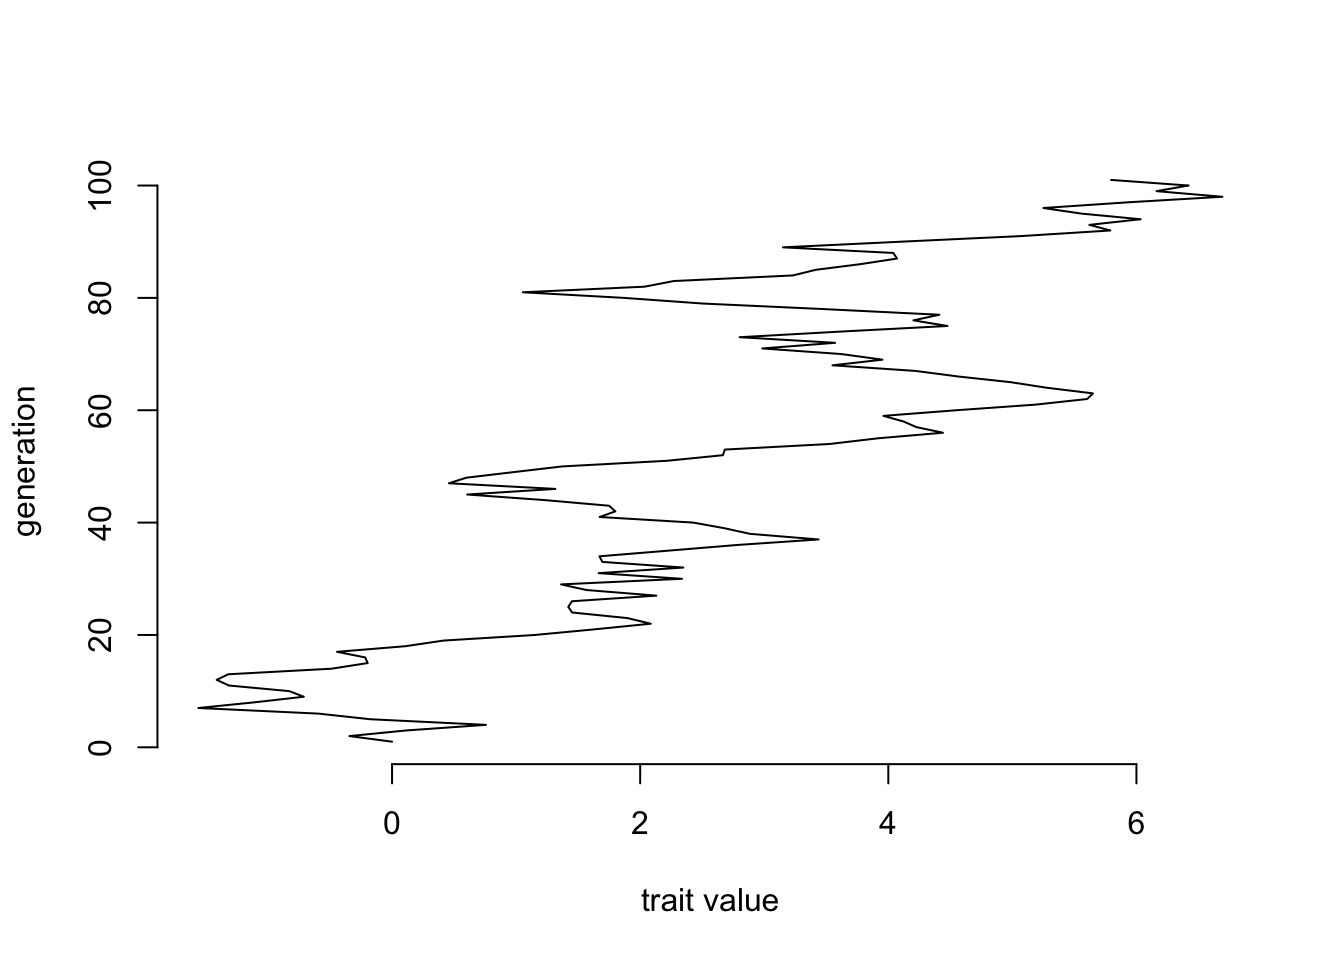
\includegraphics{comparative-methods_files/figure-latex/unnamed-chunk-9-1.pdf}

Note that this tree is a chronogram.

Let's simulate data on this tree. But what model to use? For now, let's assume we are looking at continuous traits, things like body size. Over evolutionary time, these probably undergo a series of changes that then get added up. A species has an average mass of 15 kg, then it goes to 15.1 kg, then 14.8 kg, and so forth. But how could those changes be distributed?

Start with a uniform distribution. Take a starting value of 0, then pick a number from -1 to 1 to add to it (in other words, \texttt{runif(n=1,\ min=-1,\ max=1)}). There are efficient ways to do this for many generations, but let's do the obvious way: a simple \texttt{for} loop. Do it for 100 generations.

\begin{Shaded}
\begin{Highlighting}[]
\NormalTok{ngen <{-}}\StringTok{ }\DecValTok{100}
\NormalTok{positions <{-}}\StringTok{ }\KeywordTok{c}\NormalTok{(}\DecValTok{0}\NormalTok{, }\KeywordTok{rep}\NormalTok{(}\OtherTok{NA}\NormalTok{,ngen))}
\ControlFlowTok{for}\NormalTok{ (i }\ControlFlowTok{in} \KeywordTok{sequence}\NormalTok{(ngen)) \{}
\NormalTok{  positions[i}\OperatorTok{+}\DecValTok{1}\NormalTok{] <{-}}\StringTok{ }\NormalTok{positions[i] }\OperatorTok{+}\StringTok{ }\KeywordTok{runif}\NormalTok{(}\DecValTok{1}\NormalTok{,}\OperatorTok{{-}}\DecValTok{1}\NormalTok{,}\DecValTok{1}\NormalTok{)}
\NormalTok{\}}
\KeywordTok{plot}\NormalTok{(}\DataTypeTok{x=}\NormalTok{positions, }\DataTypeTok{y=}\KeywordTok{sequence}\NormalTok{(}\KeywordTok{length}\NormalTok{(positions)), }\DataTypeTok{xlab=}\StringTok{"trait value"}\NormalTok{, }\DataTypeTok{ylab=}\StringTok{"generation"}\NormalTok{, }\DataTypeTok{bty=}\StringTok{"n"}\NormalTok{, }\DataTypeTok{type=}\StringTok{"l"}\NormalTok{)}
\end{Highlighting}
\end{Shaded}

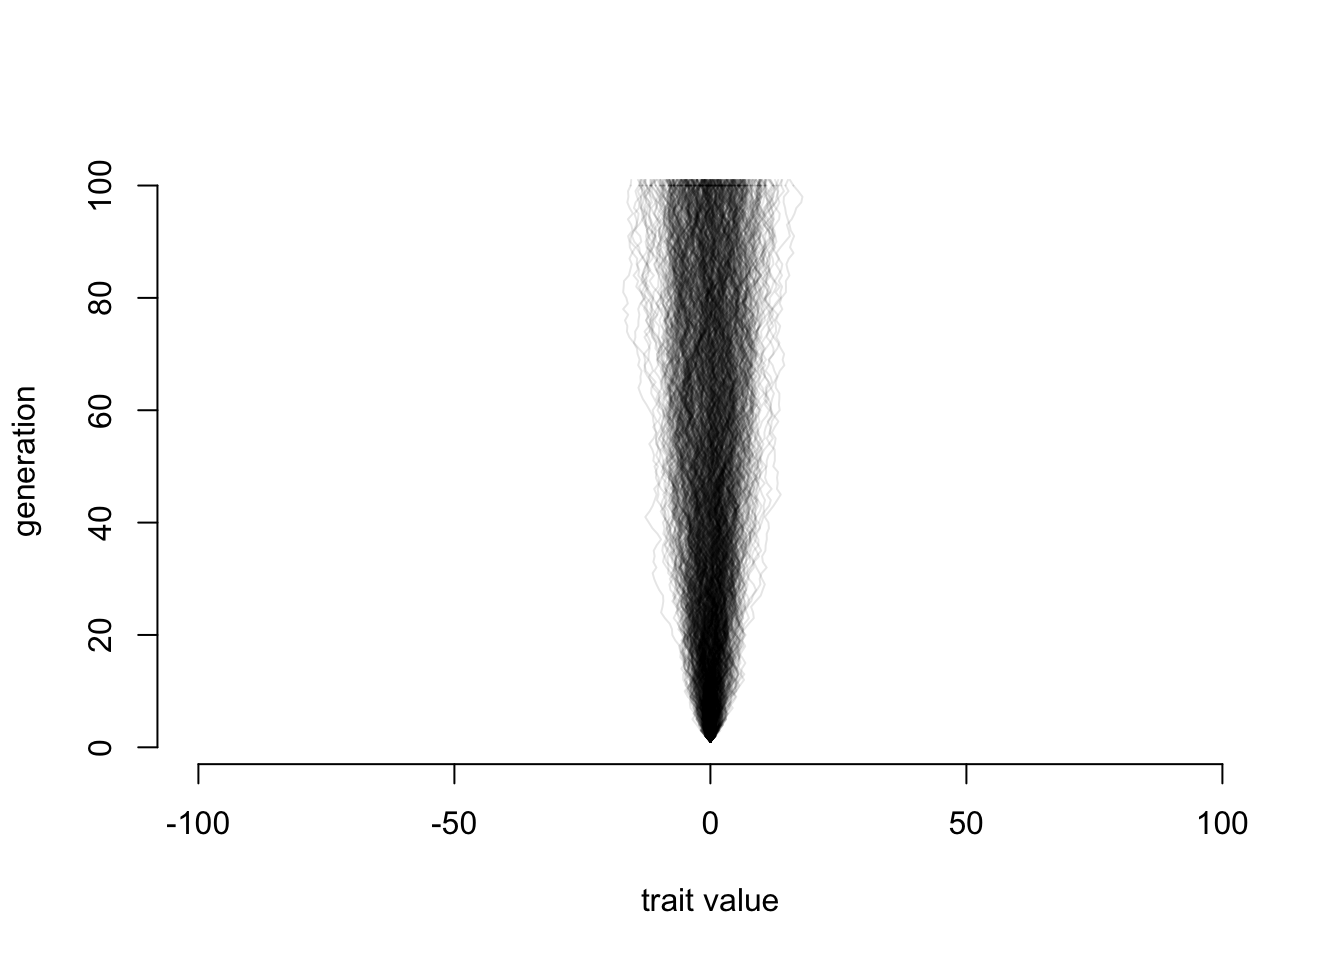
\includegraphics{comparative-methods_files/figure-latex/unnamed-chunk-10-1.pdf}

We can repeat this simulation many times and see what the pattern looks like:

\begin{Shaded}
\begin{Highlighting}[]
\NormalTok{ngen <{-}}\StringTok{ }\DecValTok{100}
\NormalTok{nsims <{-}}\StringTok{ }\DecValTok{500}
\NormalTok{final.positions <{-}}\StringTok{ }\KeywordTok{rep}\NormalTok{(}\OtherTok{NA}\NormalTok{, nsims)}
\CommentTok{\# make a plot to hold our lines}
\KeywordTok{plot}\NormalTok{(}\DataTypeTok{x=}\KeywordTok{c}\NormalTok{(}\OperatorTok{{-}}\DecValTok{1}\NormalTok{,}\DecValTok{1}\NormalTok{)}\OperatorTok{*}\NormalTok{ngen, }\DataTypeTok{y=}\KeywordTok{c}\NormalTok{(}\DecValTok{1}\NormalTok{, }\DecValTok{1}\OperatorTok{+}\NormalTok{ngen), }\DataTypeTok{xlab=}\StringTok{"trait value"}\NormalTok{, }\DataTypeTok{ylab=}\StringTok{"generation"}\NormalTok{, }\DataTypeTok{bty=}\StringTok{"n"}\NormalTok{, }\DataTypeTok{type=}\StringTok{"n"}\NormalTok{)}
\ControlFlowTok{for}\NormalTok{ (sim.index }\ControlFlowTok{in} \KeywordTok{sequence}\NormalTok{(nsims)) \{}
\NormalTok{  positions <{-}}\StringTok{ }\KeywordTok{c}\NormalTok{(}\DecValTok{0}\NormalTok{, }\KeywordTok{rep}\NormalTok{(}\OtherTok{NA}\NormalTok{,ngen))}
  \ControlFlowTok{for}\NormalTok{ (i }\ControlFlowTok{in} \KeywordTok{sequence}\NormalTok{(ngen)) \{}
\NormalTok{    positions[i}\OperatorTok{+}\DecValTok{1}\NormalTok{] <{-}}\StringTok{ }\NormalTok{positions[i] }\OperatorTok{+}\StringTok{ }\KeywordTok{runif}\NormalTok{(}\DecValTok{1}\NormalTok{,}\OperatorTok{{-}}\DecValTok{1}\NormalTok{,}\DecValTok{1}\NormalTok{)}
\NormalTok{  \}}
  \KeywordTok{lines}\NormalTok{(positions, }\KeywordTok{sequence}\NormalTok{(}\KeywordTok{length}\NormalTok{(positions)), }\DataTypeTok{col=}\KeywordTok{rgb}\NormalTok{(}\DecValTok{0}\NormalTok{,}\DecValTok{0}\NormalTok{,}\DecValTok{0}\NormalTok{,}\FloatTok{0.1}\NormalTok{))}
\NormalTok{  final.positions[sim.index] <{-}}\StringTok{ }\NormalTok{positions[}\KeywordTok{length}\NormalTok{(positions)]}
\NormalTok{\}}
\end{Highlighting}
\end{Shaded}

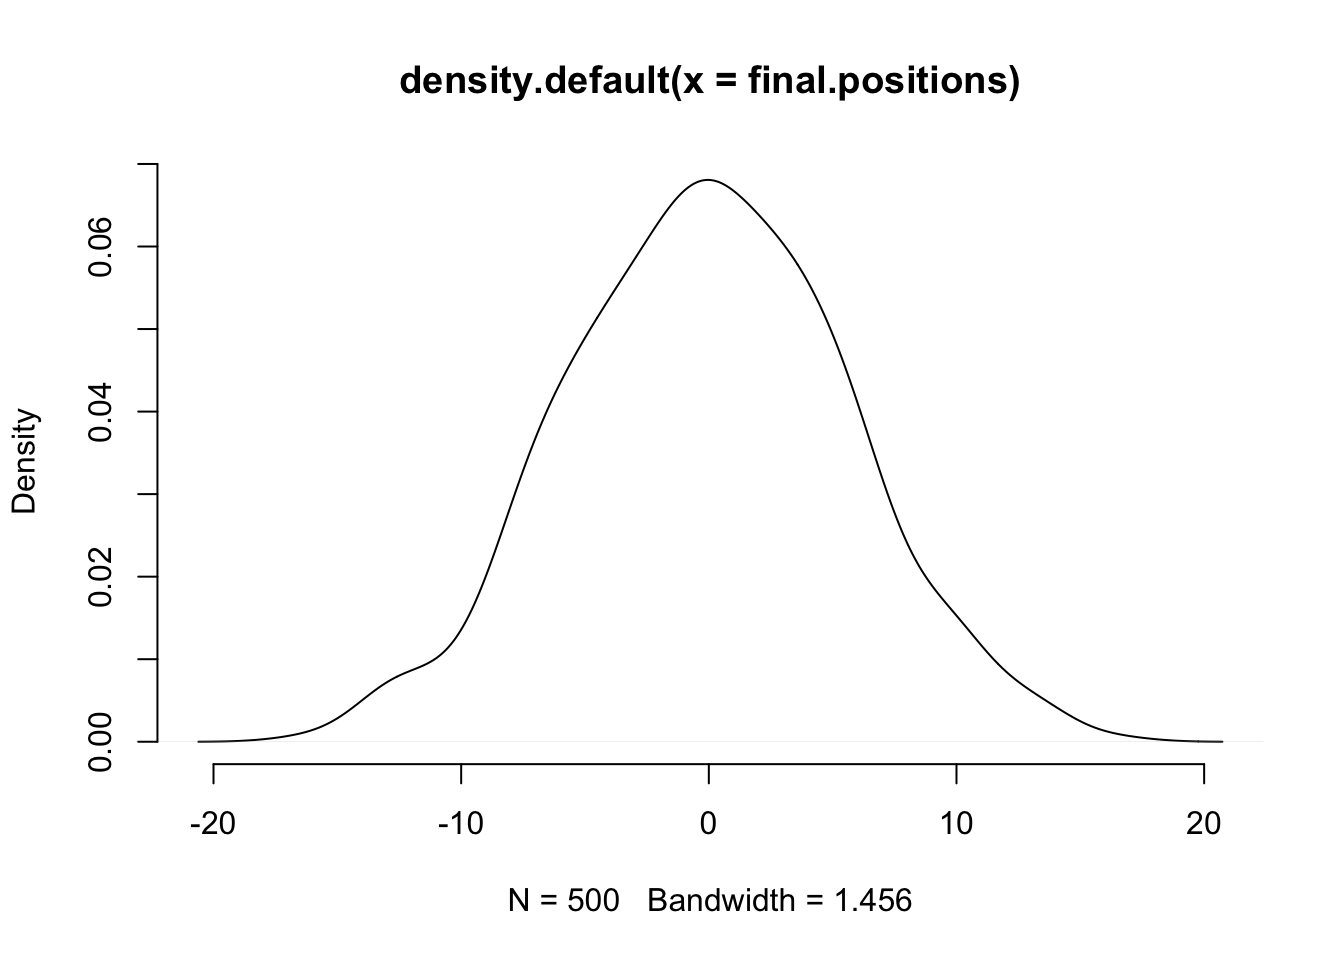
\includegraphics{comparative-methods_files/figure-latex/unnamed-chunk-11-1.pdf}

Well, that may seem odd: we're adding a bunch of uniform random values between -1 and 1 (so, a flat distribution) and we get something that definitely has more lines ending up in the middle than further out. Look just at the distribution of final points:

\begin{Shaded}
\begin{Highlighting}[]
\KeywordTok{plot}\NormalTok{(}\KeywordTok{density}\NormalTok{(final.positions), }\DataTypeTok{col=}\StringTok{"black"}\NormalTok{, }\DataTypeTok{bty=}\StringTok{"n"}\NormalTok{)}
\end{Highlighting}
\end{Shaded}

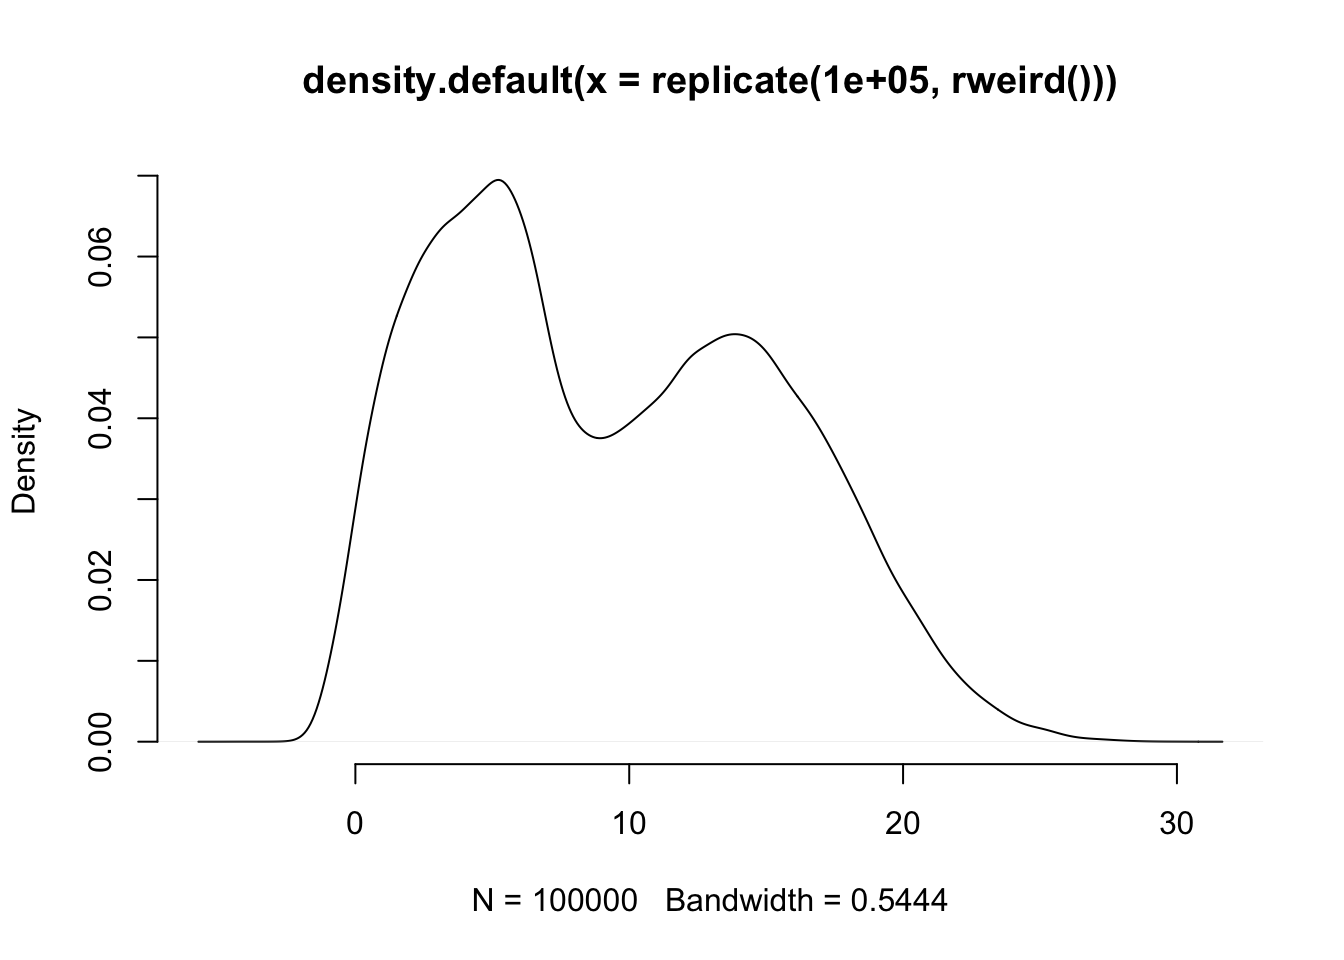
\includegraphics{comparative-methods_files/figure-latex/unnamed-chunk-12-1.pdf}

Which looks almost normal. Ok, let's try a weird distribution:

\begin{Shaded}
\begin{Highlighting}[]
\NormalTok{rweird <{-}}\StringTok{ }\ControlFlowTok{function}\NormalTok{() \{}
\NormalTok{  displacement <{-}}\StringTok{ }\DecValTok{0}
  \ControlFlowTok{if}\NormalTok{(}\KeywordTok{runif}\NormalTok{(}\DecValTok{1}\NormalTok{,}\OperatorTok{{-}}\DecValTok{2}\NormalTok{,}\DecValTok{2}\NormalTok{) }\OperatorTok{<}\StringTok{ }\FloatTok{.1}\NormalTok{) \{}
\NormalTok{    displacement <{-}}\StringTok{ }\KeywordTok{rnorm}\NormalTok{(}\DecValTok{1}\NormalTok{, }\DecValTok{7}\NormalTok{, }\DecValTok{3}\NormalTok{) }\OperatorTok{+}\StringTok{ }\KeywordTok{runif}\NormalTok{(}\DecValTok{1}\NormalTok{,}\DecValTok{0}\NormalTok{,}\DecValTok{7}\NormalTok{)}
\NormalTok{  \} }\ControlFlowTok{else}\NormalTok{ \{}
\NormalTok{    displacement <{-}}\StringTok{ }\FloatTok{0.5} \OperatorTok{*}\StringTok{ }\KeywordTok{rexp}\NormalTok{(}\DecValTok{1}\NormalTok{, }\FloatTok{0.3}\NormalTok{) }\OperatorTok{{-}}\StringTok{ }\DecValTok{1}
\NormalTok{  \}}
\NormalTok{  displacement <{-}}\StringTok{ }\NormalTok{displacement }\OperatorTok{+}\StringTok{ }\KeywordTok{round}\NormalTok{(}\KeywordTok{runif}\NormalTok{(}\DecValTok{1}\NormalTok{,}\DecValTok{1}\NormalTok{,}\DecValTok{100}\NormalTok{) }\OperatorTok{\%\%}\StringTok{ }\DecValTok{7}\NormalTok{)}
  \KeywordTok{return}\NormalTok{(displacement)  }
\NormalTok{\}}

\KeywordTok{plot}\NormalTok{(}\KeywordTok{density}\NormalTok{(}\KeywordTok{replicate}\NormalTok{(}\DecValTok{100000}\NormalTok{, }\KeywordTok{rweird}\NormalTok{())), }\DataTypeTok{bty=}\StringTok{"n"}\NormalTok{)}
\end{Highlighting}
\end{Shaded}

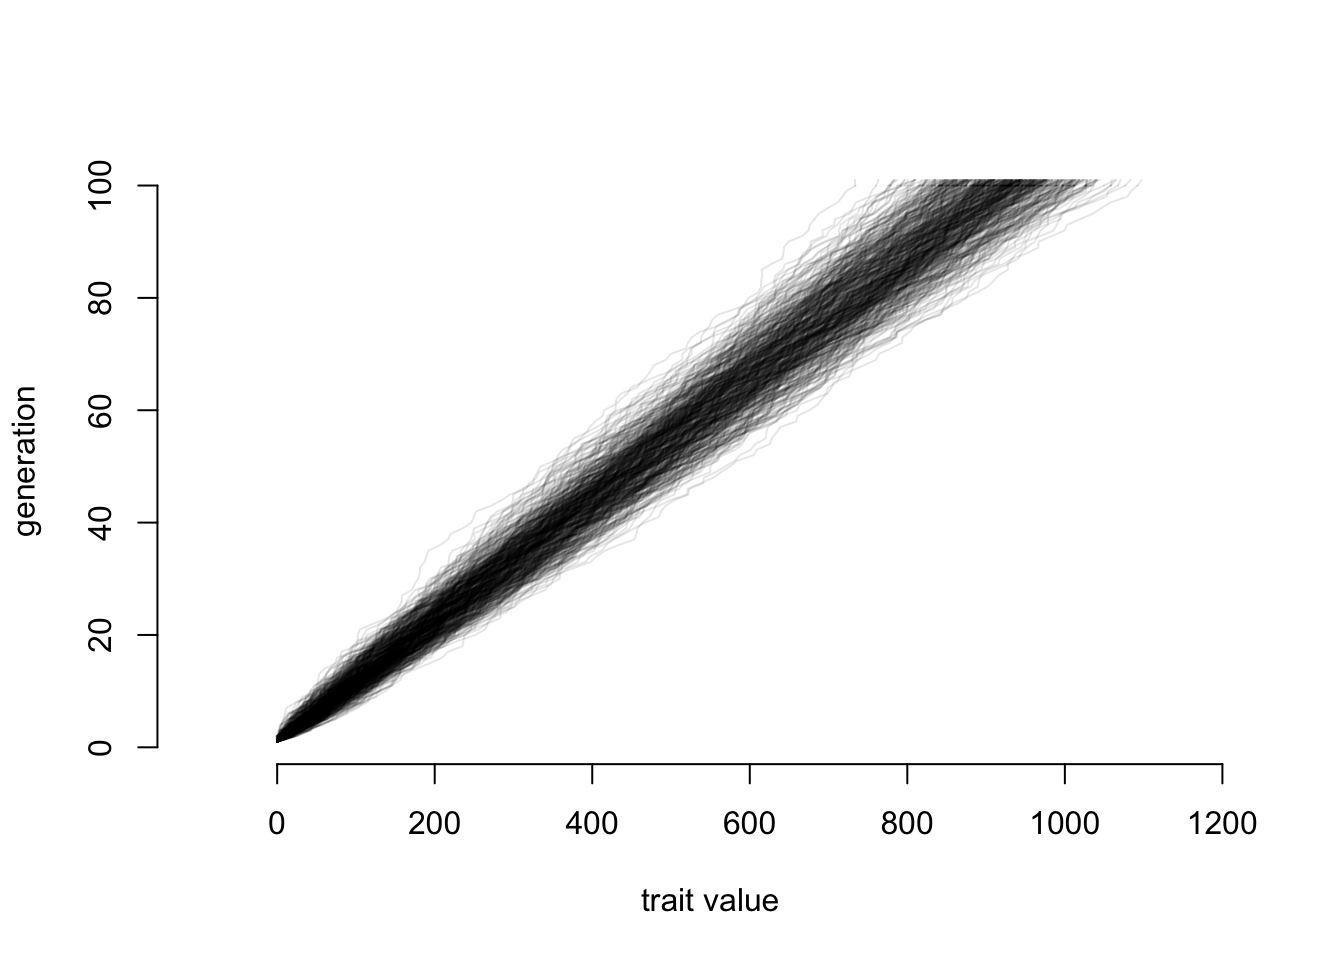
\includegraphics{comparative-methods_files/figure-latex/unnamed-chunk-13-1.pdf}

When we ask \texttt{rweird()} for a number it sometimes gives us a normally distributed number multiplied by a unifor distribution, other times it gives us an exponentially distributed number, and then adds the remainder that comes when you divide a random number by 7. So, not exactly a simple distribution like uniform, normal, or Poisson. So, repeating the simulation above but using this funky distribution:

\begin{Shaded}
\begin{Highlighting}[]
\NormalTok{ngen <{-}}\StringTok{ }\DecValTok{100}
\NormalTok{nsims <{-}}\StringTok{ }\DecValTok{500}
\NormalTok{final.positions <{-}}\StringTok{ }\KeywordTok{rep}\NormalTok{(}\OtherTok{NA}\NormalTok{, nsims)}
\CommentTok{\# make a plot to hold our lines}
\KeywordTok{plot}\NormalTok{(}\DataTypeTok{x=}\KeywordTok{c}\NormalTok{(}\OperatorTok{{-}}\DecValTok{100}\NormalTok{,}\DecValTok{1200}\NormalTok{), }\DataTypeTok{y=}\KeywordTok{c}\NormalTok{(}\DecValTok{1}\NormalTok{, }\DecValTok{1}\OperatorTok{+}\NormalTok{ngen), }\DataTypeTok{xlab=}\StringTok{"trait value"}\NormalTok{, }\DataTypeTok{ylab=}\StringTok{"generation"}\NormalTok{, }\DataTypeTok{bty=}\StringTok{"n"}\NormalTok{, }\DataTypeTok{type=}\StringTok{"n"}\NormalTok{)}
\ControlFlowTok{for}\NormalTok{ (sim.index }\ControlFlowTok{in} \KeywordTok{sequence}\NormalTok{(nsims)) \{}
\NormalTok{  positions <{-}}\StringTok{ }\KeywordTok{c}\NormalTok{(}\DecValTok{0}\NormalTok{, }\KeywordTok{rep}\NormalTok{(}\OtherTok{NA}\NormalTok{,ngen))}
  \ControlFlowTok{for}\NormalTok{ (i }\ControlFlowTok{in} \KeywordTok{sequence}\NormalTok{(ngen)) \{}
\NormalTok{    positions[i}\OperatorTok{+}\DecValTok{1}\NormalTok{] <{-}}\StringTok{ }\NormalTok{positions[i] }\OperatorTok{+}\StringTok{ }\KeywordTok{rweird}\NormalTok{()}
\NormalTok{  \}}
  \KeywordTok{lines}\NormalTok{(positions, }\KeywordTok{sequence}\NormalTok{(}\KeywordTok{length}\NormalTok{(positions)), }\DataTypeTok{col=}\KeywordTok{rgb}\NormalTok{(}\DecValTok{0}\NormalTok{,}\DecValTok{0}\NormalTok{,}\DecValTok{0}\NormalTok{,}\FloatTok{0.1}\NormalTok{))}
\NormalTok{  final.positions[sim.index] <{-}}\StringTok{ }\NormalTok{positions[}\KeywordTok{length}\NormalTok{(positions)]}
\NormalTok{\}}
\end{Highlighting}
\end{Shaded}

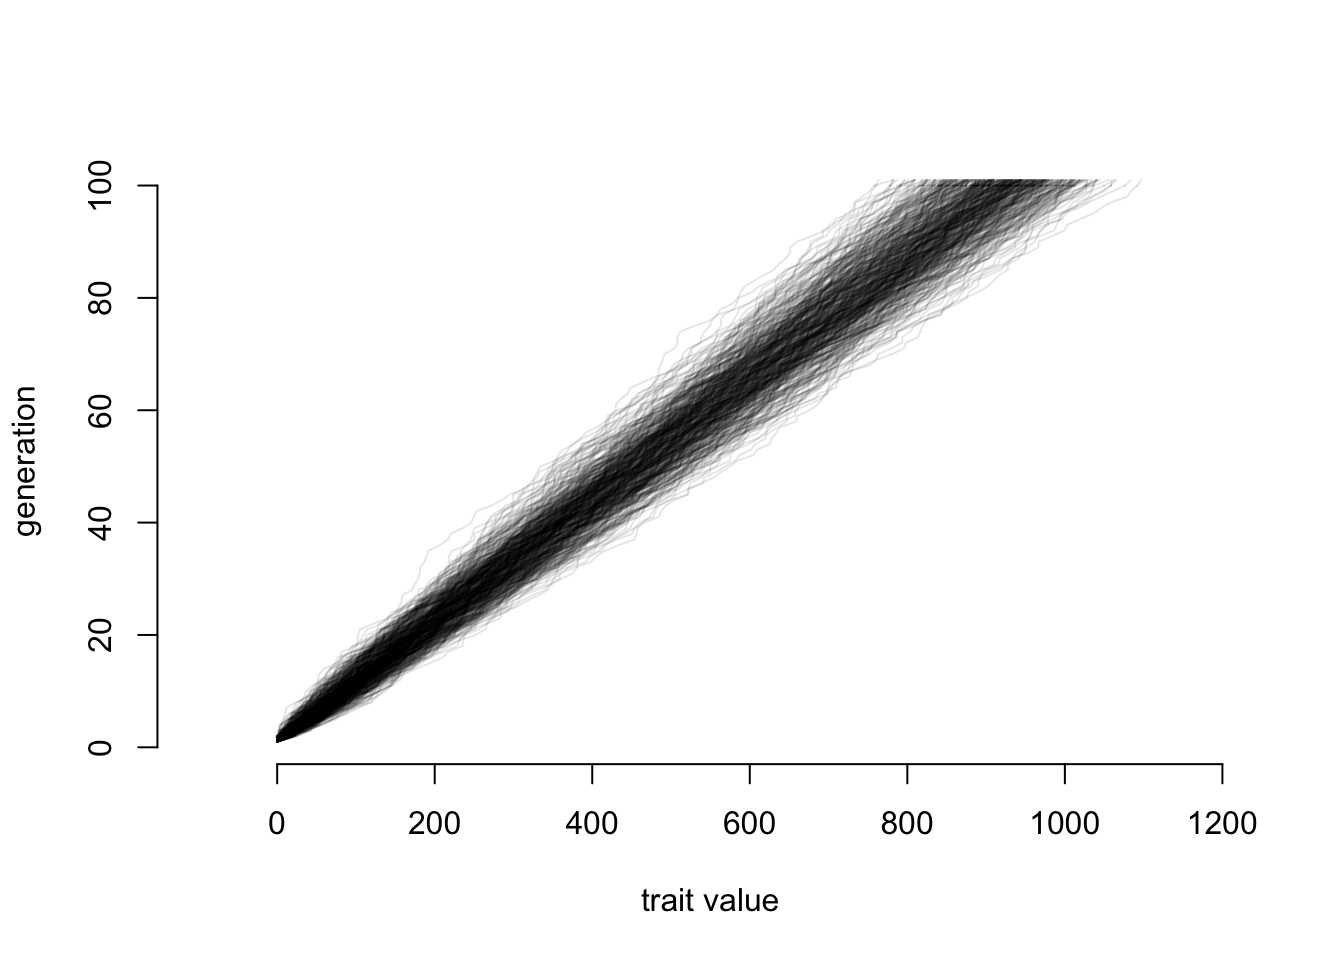
\includegraphics{comparative-methods_files/figure-latex/unnamed-chunk-14-1.pdf}

And now let's look at final positions again:

\begin{Shaded}
\begin{Highlighting}[]
\KeywordTok{plot}\NormalTok{(}\KeywordTok{density}\NormalTok{(final.positions), }\DataTypeTok{col=}\StringTok{"black"}\NormalTok{, }\DataTypeTok{bty=}\StringTok{"n"}\NormalTok{)}
\end{Highlighting}
\end{Shaded}

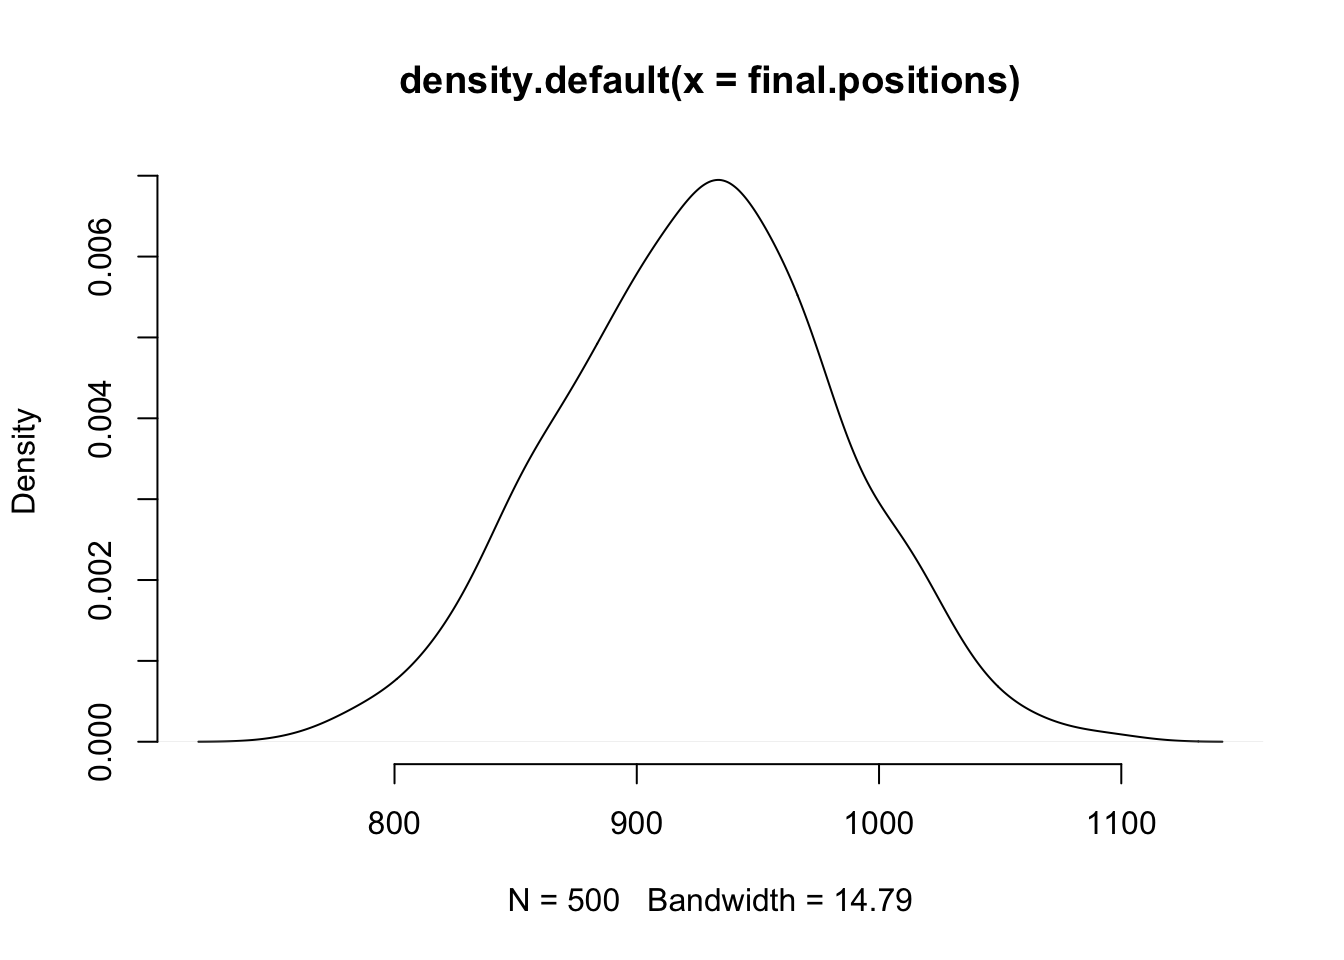
\includegraphics{comparative-methods_files/figure-latex/unnamed-chunk-15-1.pdf}

Again, it looks pretty much like a normal distribution. You can try with your own wacky distribution, and this will almost always happen (as long as the distribution has finite variance).

Why?

Well, think back to stats: why do we use the normal distribution for so much?

Answer: the central limit theorem. The sum (or, equivalently, average) of a set of numbers pulled from distributions that each have a finite mean and finite variance will approximate a normal distribution. The numbers could all be independent and come from the same probability distribution (i.e., could take numbers from the same Poisson distribution), but this isn't required.

Biologically, the technical term for this is awesome. We know something like a species mean changes for many reasons: chasing an adaptive peak here, drifting there, mutation driving a it this way or that, etc. If there are enough shifts, where a species goes after many generations is normally distributed. For two species, there's one normal distribution for their evolution from the origin of life (or the start of the tree we're looking at) to their branching point (so they have identical history up to then) then each evolves from that point independently (though of course in reality they may interact; the method that's part of the grant supporting this course allows for this). So they have covariance due to the shared history, then accumulate variance independently after the split. We thus use a multivariate normal for multiple species on the tree (for continuous traits), but it again is due to Brownian motion. \textbf{This mixture of independent and shared evolution is quite important: it explains why species cannot be treated as independent data points, necessitating the correlation methods that use a phylogeny in this week's lessons.}

However, in biological data there are (at least) two issues. One is that in some ways a normal distribution is weird: it says that for the trait of interest, there's a positive probability for any value from negative infinity to positive infinity. ``Endless forms most beautiful and most wonderful have been, and are being, evolved'' {[}Darwin{]} but nothing is so wonderful as to have a mass of -15 kg (or, for that matter, 1e7 kg). Under Brownian motion, we expect a displacement of 5 g to have equal chance no matter what the starting mass, but in reality a shrew species that has an average mass of 6 g is less likely to lose 5 g over one million years than a whale species that has an average adult mass of 100,000,000 g. Both difficulties go away if we think of the displacements not coming as an addition or subtraction to a species' state but rather a multiplying of a state: the chance of a whale or a shrew increasing in mass by 1\% per million years may be the same, even if their starting mass magnitudes are very different. Conveniently, this also prevents us getting zero or lower for a mass (or other trait being examined). This works if we use the \textbf{log of the species trait and treat that as evolving under Brownian motion}, and this is why traits are commonly transformed in this way in phylogenetics (as well they should be).

The other issue is that the normal approximation might not hold. For example, if species are being pulled back towards some fixed value, the net displacement is not a simple sum of the displacements: we keep getting pulled back, in effect eroding the influence of movements the deeper they are in the past: thus the utility of Ornstein-Uhlenbeck models. There may also be a set of displacements that all come from one model, then a later set of displacements that all come from some different model: we could better model evolution, especially correlation between species, by using these two (or more) models rather than assume the same normal distribution throughout time: thus the utility of approaches that allow different parameters or even different models on different parts of the tree.

\hypertarget{correlation}{%
\subsection{Correlation}\label{correlation}}

For this week, bring your data and a tree for those taxa. Fork \url{https://github.com/PhyloMeth/Correlation} and then add scripts there. When you're done, do a pull request. Note if you add data to that directory and commit it, it'll be uploaded to public GitHub. Probably not a big deal, unless you want to keep your data secret and safe (Lord of The Rings reference; c.f. \texttt{phangorn} package).

\textbf{Do independent contrasts} using \texttt{pic()} in \texttt{ape}. Remember to 1) positivize the contrasts (this is \emph{not} the same as doing \texttt{abs()}). From the Garland et al.~paper, think about ways to see if there are any problems. How do contrasts affect the correlations?

\textbf{Do Pagel94}
There are at least three ways to do this in R: in the \texttt{phytools}, \texttt{diversitree}, and \texttt{corHMM} packages. With \texttt{phytools}, it's pretty simple: use the \texttt{fitPagel()} function. With the others, you have to specify the constraint matrices (this allows you to do Pagel-style tests but on a wider range of models). Think about what you should assume at the root state: canonical Pagel94 assumes equal probabilities of each state at the root, but that might be a bad assumption for your taxa.

\textbf{Use another correlation method}
Perhaps phyloGLM? Use the \texttt{phylolm} package, or some other approach to look at correlations.

\hypertarget{discrete-traits}{%
\section{Discrete Traits}\label{discrete-traits}}

\#\#Objectives

By the end of this chapter, you will:

\begin{itemize}
\tightlist
\item
  Understand how to incorporate rate heterogeneity in discrete trait models
\item
  Be able to explain how to test hypotheses about univariate trait evolution.
\end{itemize}

Many traits can be thought of as discrete traits: a DNA site comes in ATGC, protein have one of 20 amino acids, some animals have functional eyes and others do not, some plants are woody and others are herbaceous. This is nearly always an approximation. Think of something like limbs: they seem distinct enough that we even name some groups by their count: tetrapods, hexapods. Except that when we look closely enough, it becomes fuzzy: insect mouthparts are derived from limbs, for example, so should we count these highly modified limbs as limbs (and if not, where in evolution have they become sufficiently modified to no longer count? And are nymphalid butterflies tetrapods under that definition yet?). Are modern whales thought to have four limbs, even though two are extremely vestigial? Often for neontologists problematic organisms with intermediate counts are conveniently extinct (so long, \emph{Basilosaurus}), so we can ignore this fuzziness, but it is often there (and paleontologists are confronted with it more often). Think about the details of a species changing from one discrete state to another, even for something like a seemingly perfectly discrete character like a base changing from an A to a T. At first this is present in just a single individual (for a multicellular diploid, on one DNA strand in one cell in the germ line). Even if under selection, it will take generations to sweep through to fixation: during that time, what is ``the'' state of the species? It is even harder to discretize characters like woodiness (how much wood is required?), eyes (when does a fish population evolving in a cave finally ``lose'' its eyes?), biogeography (how finely do you divide the range: by continent? biome? state?), and so forth.

As for many decisions, this comes back to the biological hypotheses being tested and the size of the study. For example, one question could be does a complex trait like wings ever re-evolve once lost? \citet{Whiting2003} examined this in stick insects: some species have wings in both sexes, some in one only, and some lack wings in both sexes. If the question hinges on whether loss of wing genes in a species prevents re-evolution, then as long as one sex in a species has wings the species should be coded as having wings. If the question hinges on the effect of loss of wings on ability to settle new areas, it could be that having either sex lack wings is enough to prevent effective colonization, and thus a species with only one sex with wings should be coded as being wingless. If the study system is large enough to have sufficient power, one could code this as a four state character, instead: \textbf{A}: both males and females have wings; \textbf{B}: males have, females lack wings; \textbf{C}: males lack, females have wings; and \textbf{D}: both males and females lack wings.

One way to deal with this is to gather discrete data as finely divided as reasonable and then aggregate. For example, in the stick insect example, code it as a four state character as above and then, depending on the biological question, group them. If the question is whether wings can reappear after being entirely lost, for example, one would group \textbf{A}, \textbf{B}, and \textbf{C} as having wings (in at least some members of the species, so the genes remain under selection for functionality) and \textbf{D} as wingless, but for the dispersal question one could lump \textbf{B}, \textbf{C}, and \textbf{D}, leaving \textbf{A} as the other state, or even lump \textbf{B} and \textbf{C} only.

\begin{tabular}{l|l|l|r|r|r}
\hline
males & females & four\_states & question\_1 & question\_2a & question\_2b\\
\hline
wings & wings & A & 1 & 1 & 2\\
\hline
wings & wingless & B & 0 & 1 & 1\\
\hline
wingless & wings & C & 0 & 1 & 1\\
\hline
wingless & wingless & D & 0 & 0 & 0\\
\hline
\end{tabular}

But, let's assume we can discretize traits and carry on. The simplest discretization is binary: 0 or 1, often absence or presence (but could be yellow or blue, etc.). Most models are like our commonly used DNA models: continuous time with discrete changes, using the same rates throughout. It is like a model for when an autonomous car will have an accident: assuming the car works perfectly (gives a whole new meaning to ``blue screen of death'') there's still a chance that at some point a human is going to run into it. There's a per hour chance of an accident: let's assume in each hour there's a 0.03\% chance of our autonomous car having an accident (very roughly based on Google's experience, assuming a 40 MPH average speed). So the probability of having no accident in the first hour of driving is 99.97\%; the probability of having no accidents in the first 40 hours of driving is 99.97\% \^{} 40 = 98.8\%. The number of accidents is Poisson-distributed; the wait time between accidents is exponentially distributed. This is the model commonly used in phylogenetics for discrete traits, though sometimes with more complexity: one could move (with some rate) between two different rates, as in a covarion model, for example. A very different model is Felsenstein's threshold model, which we will discuss in a few weeks. For now, though, just envision models with a fixed rate of change between states as long as other characters don't change; it's possible, though, that the state of other characters do affect these rates (which is what correlation tests investigate). For example, the probability of switching from clawed feet to flippers for forelimbs is probably much higher for species that live in water than on land.

(btw, note the spelling here: having one, two or eight eyes is a \emph{discrete} trait: individually separate and distinct. Forming an enclosed bower for hidden mating is a \emph{discreet} trait. The former is generally far more biologically relevant).

Discrete trait models typically assume that change from one state to another happens in one step. Time is continuous (per instant, rather than change per generation, per year, etc.). Usually the process is memoryless: there's no cooling-off period during which a trait can't change back, for example (there are seeming exceptions, like the threshold model \citep{felsenstein_comparative_2012}, though these often are memoryless when you look more deeply (like in the liability in the threshold model)). This memoryless property makes this a Markovian model. So, overall, these are discrete state continuous time Markov chain models (DSCTMC) \citep{omeara_evolutionary_2012-1}. When in one state, there's an exponentially distributed wait time until a change to some other state. An example of this is radioactive decay: an atom of carbon-14 sitting patiently in a sugar molecule, until at some point it decays to form a nitrogen atom. It might happen in a second, it may happen in 100 years, it may happen in 10,000 years. The faster the decay rate, the less time on average until it changes. For atomic decay, we often talk about half life (1/rate): this can be done for phylogenetics, too {[}note this is distinct from phylogenetic half life for Ornstein-Uhlenbeck models -- see that chapter{]}. This can give an intuitive sense of time to a change: is there a 50:50 chance the trait has changed after 10 MY (reasonable) or after 0.0001 years (seems a bit fast for most traits)?

It's possible a trait can have more than two states. Take DNA: an A could change to a T, to a G, or to a C. There could be three rates: r\textsubscript{AT}, r\textsubscript{AG}, r\textsubscript{AC} for changes from A to T, A to G, and A to C respectively. The rate it changes at all is the sum of these: r\textsubscript{A\_} = r\textsubscript{AT} + r\textsubscript{AG} + r\textsubscript{AC}. The probability that the change is A to T when it does change is just r\textsubscript{AT} / (r\textsubscript{AT} + r\textsubscript{AG} + r\textsubscript{AC}).

It is often convenient to arrange the instantaneous rates into a table. Each row represents a starting state, and each column represents an ending state. Each cell is the instantaneous rate of going from the row state to the column state:

\begin{tabular}{l|l|l|l|l}
\hline
  & A & T & G & C\\
\hline
A & - & r\textasciitilde{}AT\textasciitilde{} & r\textasciitilde{}AG\textasciitilde{} & r\textasciitilde{}AC\textasciitilde{}\\
\hline
T & r\textasciitilde{}TA\textasciitilde{} & - & r\textasciitilde{}TG\textasciitilde{} & r\textasciitilde{}TC\textasciitilde{}\\
\hline
G & r\textasciitilde{}GA\textasciitilde{} & r\textasciitilde{}GT\textasciitilde{} & - & r\textasciitilde{}GC\textasciitilde{}\\
\hline
C & r\textasciitilde{}CA\textasciitilde{} & r\textasciitilde{}CT\textasciitilde{} & r\textasciitilde{}CG\textasciitilde{} & -\\
\hline
\end{tabular}

Though the above example is for DNA, one could do the same with amino acids, ability to fly, having eyes, growth form, trophic level, etc.

Once we have this matrix, we can do a few cool things with it. One is to calculate the probability of starting in one state and ending in a particular state over some time \emph{t}. This is frankly amazing: think of the ways one could start in A and end in T. One could change from A to T exactly at the middle of the time interval. Or, this could happen 10\% of the way along the branch. Or, one could change from A to G a third of the way up and then G to T a bit further along. Or could go from A to T to A to T. Etc. There are an infinite number of paths one could take to get from A to T. However, by simply taking the instantaneous rate matrix, \textbf{Q}, multiplying each cell by \emph{t}, and taking the matrix exponential of this, we can integrate over \emph{all} these paths to get the probability matrix \textbf{P}, where the entry for row \emph{i}, column \emph{j} is the probability of starting in state \emph{i} and ending in state \emph{j} over time \emph{t}.

With a way to calculate probability, all manner of wondrous things become available. For example, take this very simple tree:

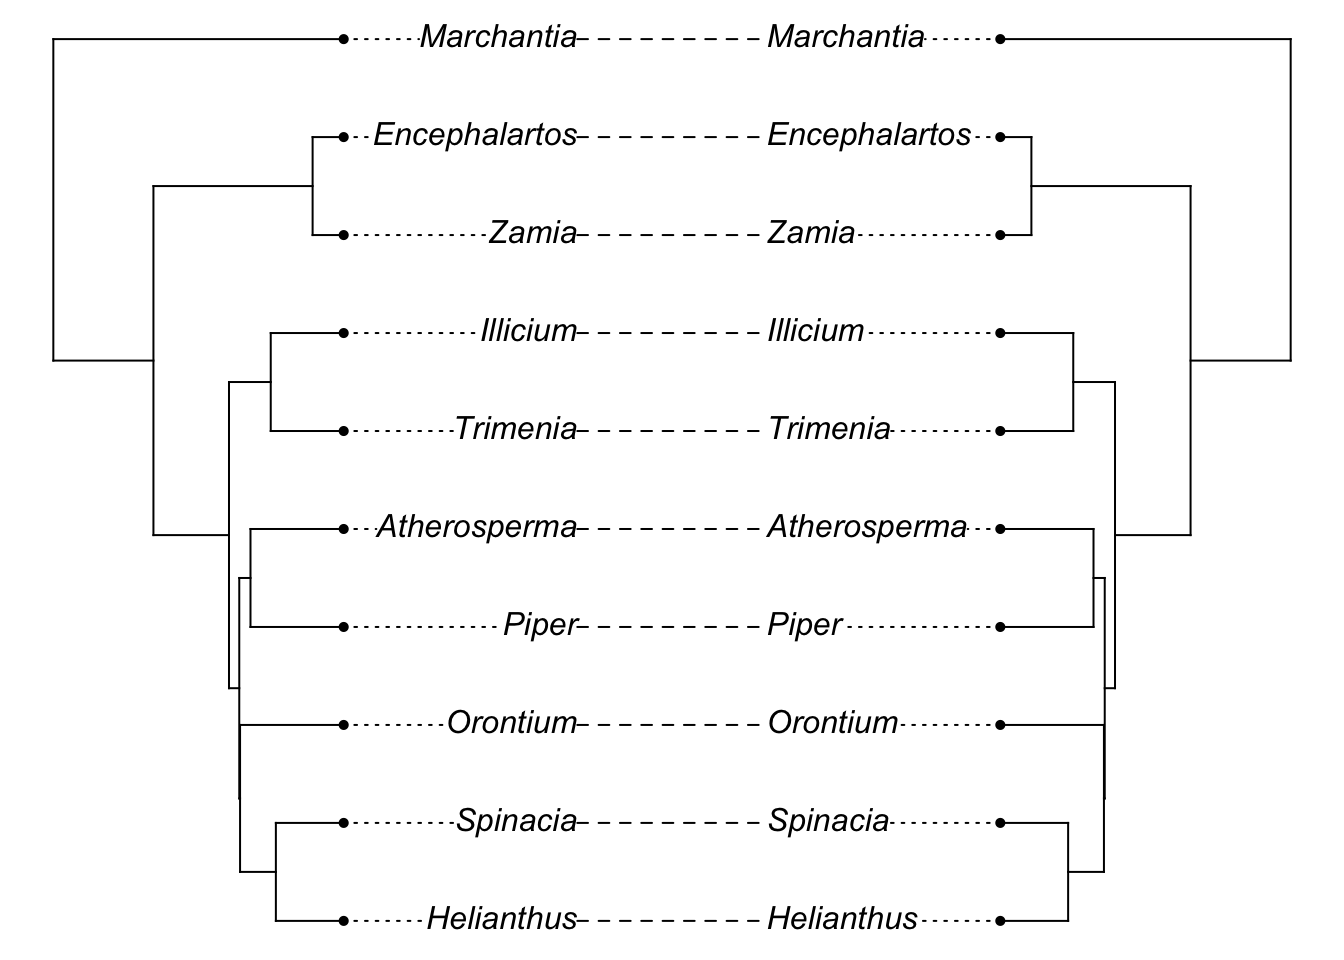
\includegraphics{comparative-methods_files/figure-latex/unnamed-chunk-18-1.pdf}

What is the probability of the data (the likelihood) of this tree? Well, we have two paths: from A at the root of the tree to A over a time of 0.7, and from A at the root of the tree to G, also over a time of 0.7. If we know the instantaneous rates, we can take the matrix \textbf{Q}, do \textbf{P} = expm(\textbf{Q} times \emph{t}), and calculate the probability of A to A and A to G paths. Multiply those two probabilities together than that is the probability of seeing A and G at the tips and A at the root given the instantneous rates: that is, we've calculated the likelihood of the tree. We could try changing the branch length from 0.7 to 0.71 or 0.69, repeat, and continue trying branch lengths until we find a branch length that maximizes this probability: that's finding the maximum likelihood optimum branch length. If we do not want to assume an A at the root, we could calculate the probability of the data assuming a T at the root, assuming an A, assuming a G, and assuming a C, weight each probability by our expectation of seeing each root state (for example, if we assume we know nothing a 1/4 chance of each state) and get the weighted sum. This is how likelihoods of trees are calculated in general. For larger trees, we essentially do the same thing, trying all possible combinations of states at each node (there's actually a faster but equivalent algorithm, known as tree pruning or tree peeling, developed by Felsenstein that's used in practice). If we want to estimate the state at one particular node (the marginal ancestral state estimate), we integrate (add) over all possible combinations of states at other nodes but trying each possible state at our focal node to find the likelihood of the data given each state -- this is ancestral state estimation. If we want to compare two different trees, we calculate the probability of the data on each tree and compare them. Combined with a way of proposing new trees, this is a likelihood tree search algorithm.

In the same way we can try different branch lengths and get different likelihoods to find the optimal branch length, we can try different rates and try to get the ones that maximize the probability of the data. Many questions relate to these rates. Is the rate of gaining eyes lower than the rate of losing eyes? To answer, find the values that maximize the likelihood, see if the gaining eyes rate is lower. It can be helpful to compare rates under a model where they are allowed to vary with models where they are forced to be the same: for example, we can set the gain rate to equal the loss rate and see how much worse that is. This is also one way we simplify models: either by forcing some paramter values to have the same rates or by forcing some rates to be a fixed value (usually zero). For example, for DNA models, a common one is to assume that the rate of going from state \emph{i} to \emph{j} is the same as going from \emph{j} to \emph{i}: this is known as a general time reversible model. This often fits almost as well as a model with all transition rates allowed to vary, but has half the number of parameters to fit. An even simpler model, the Jukes-Cantor model, forces all rates from one nucleotide to another to be equal. One can also ask about direction of transitions: is it always 0 -\textgreater{} 1 -\textgreater{} 2, or are 0 -\textgreater{} 2 changes possible directly? To examine this, compare models with r\textsubscript{02} forced to be zero and see how much worse they are than models with unconstrained rates.

Ancestral state estimation is a common desire for biologists. There are multiple ways to estimate these states. The first question is where the states are estimated (adopting the jargon of \citet{steel_parsimony_2000}). The likelihood calculated by averaging across all states everywhere (except terminals), as we do when finding the best tree, is known as maximum average likelihood. For ancestral state estimation, it is typical to estimate states at nodes: this is known as most-parsimonious likelihood. Note that estimating states at the nodes takes two forms. The less common, but which is the one matching the most-parsimonious likelihood approach, is a joint reconstruction: find the set of states across all nodes that together maximize the likelihood. It's like asking what your favorite meal is: maybe a hot dog, with mustard, on a grilled bun with a side of potato salad and a side of baked beans. More common is a marginal reconstruction: estimate the best state at each node, averaging across all other states at other nodes. It's equivalent to asking about your favorite food: perhaps cheddar cheese. One can do this at every node, and plot them all on the tree, but there's no guarantee that they will all be the best combined meal (cheese at one node, chocolate at another\ldots), only that each is best at its own node. In practice the two reconstructions are often very similar. A third way, which is what many of us want but which is hard in practice, is pathway likelihood: get the best state at every time point (including along branches) along the tree. That'd be great: we could see if a trait in a mammal lineage evolved before or after nonavian dinodaurs went extinct, for example. However, we don't do it in practice (one reason could be that the maximum likelihood estimates are fairly boring: depending on rates, a change will happen at the very beginning, very end, or equally likely anywhere). Instead, stochastic character mapping is often used \citep{huelsenbeck_stochastic_2003}

\hypertarget{diversification}{%
\section{Diversification}\label{diversification}}

\hypertarget{objectives-4}{%
\subsection{Objectives}\label{objectives-4}}

By the end of this chapter, you will:

\begin{itemize}
\tightlist
\item
  Understand diversification models that don't incorporate traits
\item
  Be able to estimate diversification parameters for your data
\end{itemize}

Make sure to \textbf{read the relevant papers}: \url{https://www.mendeley.com/groups/8111971/phylometh/papers/added/0/tag/diversification/}

And \textbf{do the relevant exercise}:
\url{https://github.com/PhyloMeth/Diversification}

\hypertarget{sse-methods}{%
\section{SSE methods}\label{sse-methods}}

\hypertarget{objectives-5}{%
\subsection{Objectives}\label{objectives-5}}

By the end of this chapter, you will:

\begin{itemize}
\tightlist
\item
  Understand models that look at the effects of traits on diversification
\item
  Understand some of the problems with these
\item
  Be able to categorize Type I and Type II errors and talk about their relevance.
\end{itemize}

Make sure to \textbf{read the relevant papers}: \url{https://www.mendeley.com/groups/8111971/phylometh/papers/added/0/tag/sse/}

At this point in the course, you should be familiar with working through getting software running. If you want more practice, you could use the \href{https://cran.r-project.org/web/packages/hisse/vignettes/hisse-vignette.html}{vignette} written by Jeremy Beaulieu for hisse; running diversitree is similar. However, I think a bigger thing to discuss is how we understand a method is working well, and how we assess whether results are believable. This is especially prominent in discussions of diversification. One great example of this discussion in the literature:

\begin{itemize}
\tightlist
\item
  \href{http://rstb.royalsocietypublishing.org/content/344/1307/77}{Nee et al.~(1994)} ``Extinction rates can be estimated from molecular phylogenies''
\item
  \href{http://onlinelibrary.wiley.com/doi/10.1111/j.1558-5646.2009.00926.x/abstract}{Rabosky (2009)} ``Extinction rates should not be estimated from molecular phylogenies''
\item
  \href{http://onlinelibrary.wiley.com/doi/10.1111/evo.12614/abstract}{Beaulieu and O'Meara (2015)} ``Extinction rates can be estimated from moderately sized molecular phylogenies''
\item
  \href{http://onlinelibrary.wiley.com/doi/10.1111/evo.12820/full}{Rabosky (2015)} ``Challenges in the estimation of extinction from molecular phylogenies: A response to Beaulieu and O'Meara''
\end{itemize}

And that probably isn't the last word on this (no, I'm not planning something at the moment). However, despite all the hemming and hawing over what people \emph{should} do, people still keep using methods: folks using \texttt{diversitree}, \texttt{BAMM}, \texttt{geiger}, or many other approaches merrily estimate extinction rates as a necessary part of their analyses, though they usually don't focus on them in their studies, instead focusing on diversification (speciation - extinction) or speciation alone. (Note: it is possible to do diversification approaches without estimating extinction rates: one could fix extinction rate at a known value (perhaps using the average duration of fossil ``species'' to get a fixed estimate), though what is usually done is to fix extinction at 0 (this is called a Yule model, if speciation is constant). This is a bit weird when you think about it: one of the few things we truly know in biology without a doubt is that extinction is far, far from zero in general (though this wasn't \href{http://www.ucmp.berkeley.edu/mammal/artio/irishelk.html}{really discovered in Western science until the 19th century})). But as skeptical scientists, we should aim higher. It's often tempting, especially as students or postdocs facing a difficult job market, to focus on what we can get out: is there an exciting result that can get past peer review and build our fame (maybe, in our tiny circle) and fortune (ha!). But it's important to take a step back: are we confident enough, truly (not just based on the p-value) that our results are actually discoveries about nature? Diversification is an area (ancestral state estimation is another) where the reality of results is especially worrisome. Take, for example, \href{http://onlinelibrary.wiley.com/doi/10.1111/2041-210X.12565/abstract}{Etienne et al.~(2016)}, who as part of a broader simulation study, analyzed a dataset of 25 \emph{Dendroica} warbler species, which is a classic dataset for these studies, fitting a logistic growth model. They found that depending on how the model was conditioned\footnote{Conditional probability is the probability of an event given that some other event has occurred. For example, you could use past information from your department to estimate \texttt{Prob(getting\ tenure)}, but it is different if you use information that another event has occurred: \texttt{Prob(getting\ tenure\ \textbar{}\ made\ major\ discovery\ in\ evolution)} is different from \texttt{Prob(getting\ tenure\ \textbar{}\ four\ years\ since\ last\ publication)}. In this domain (diversification alone and diversification plus trait models), we condition on actually having a tree to look at: if the true model is speciation rate equals extinction rate, there's a good chance that most clades starting X million years ago will have gone extinct, so the ones we see diversified unusually quickly, and this has to be taken into account. The example I usually use for this is the idea that dolphins rescue drowning sailors. It's known dolphins push interesting objects in the ocean. We could interview previously drowning sailors that dolphins pushed towards shore, and they'll all say that dolphins saved them, but it's very hard to interview sailors the dolphins pushed the other way. As always, Randall Munroe's XKCD explains conditional probability best
  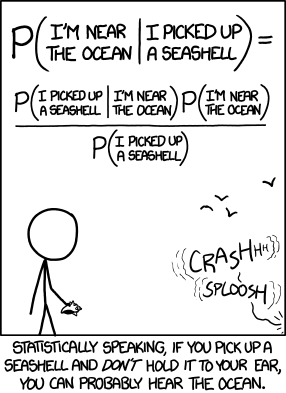
\includegraphics{images/seashell.png}}, something most users would ignore, the estimated carrying capacity (in this model, the number of warbler species at which speciation equals extinction; in other models, this would be the number of species at which speciation is zero, with extinction \emph{always} set to zero) for warblers is 24.59 or 6.09 or 0.656 species. That means, depending on how one conditions, we should expect the number of \emph{Dendroica} warblers to stay exactly where it is, crash to around six species, or crash to half a species {[}and of course, in the latter two cases, stochastic change in number of species will lead to them hitting zero species fairly quickly, which is an absorbing state{]}. Given the sensitivity of the model to factors like conditioning, any result has to be taken with a great deal of skepticism.

For trait based models, the same history of finding problems and the solutions (or partial solutions) has arisen (there is a paper coming out in the \emph{American Journal of Botany} in May 2016 that goes into this in more detail). The most relevant parts:

\href{http://onlinelibrary.wiley.com/doi/10.1111/j.0014-3820.2006.tb00517.x/abstract}{Maddison (2006)} (and there were similar points made by others earlier) showed that transition rates and diversification rates can be hard to distinguish. Oversimplifying a bit, but if the rate of going from state 0 to state 1 is higher than the reverse rate, then over time there should be many more taxa in state 1 than 0. If the diversification rate in state 1 is higher than in state 0, there will tend to be more taxa in state 1 than 0. So if you see a tree with more state 1 than 0, is it higher transition rate to 1, or higher diversification in 1? Or is it lower transition to 1 but a high enough diversification rate that it overwhelms it? Or just chance? The paper identified the problem but not the solution: the last line of the abstract is ``Studies of biased diversification and biased character change need to be unified by joint models and estimation methods, although how successfully the two processes can be teased apart remains to be seen.''

This was followed up by \href{http://sysbio.oxfordjournals.org/content/56/5/701.short}{Maddison et al.~(2007)} who figured out a method to deal with this: BiSSE. And systematists looked at it, and it was good. There is now a bestiary of similar *SSE models for different kinds of data: QuaSSE, GeoSSE, MuSSE, ClaSSE, and more.

However, there are concerns. The original paper showed that estimating extinction was hard to do accurately, and other papers (Davis et al, 2013) showed that you needed a hundreds of species to find significant results (sorry, \emph{Dendroica} -- you will forever remain a mystery). However, a particular scary paper (and talk at Evolution, where it was presented) was \href{https://sysbio.oxfordjournals.org/content/early/2014/10/23/sysbio.syu070.full}{Maddison \& FitzJohn (2014)}. Their paper mostly discussed correlated characters, but has relevance to SSE approaches. If you have a single change on a tree, you don't know if a higher rate in the clade descended from that branch is due to that trait, some other trait changing on that branch, or some other trait changing on the tree but in a way that makes it mostly on one part of the tree. \href{http://sysbio.oxfordjournals.org/content/early/2015/01/18/sysbio.syu131}{Rabosky \& Goldberg (2015)} showed that the way many people interpret BiSSE results, as a testing of a null hypothesis, can be misled if part of the null hypothesis is wrong but not the part you're interested in. \href{http://sysbio.oxfordjournals.org/content/early/2016/03/25/sysbio.syw022.abstract}{Beaulieu \& O'Meara (2016)} address some of the Maddison \& FitzJohn issues (a character changing elsewhere on the tree driving a result) but not all the issues (a single change being sufficient to give substantial support for an idea that that trait is driving diversification).

\hypertarget{discussion-prompts}{%
\subsubsection{Discussion prompts}\label{discussion-prompts}}

\begin{enumerate}
\def\labelenumi{\arabic{enumi}.}
\tightlist
\item
  What is Type I and Type II error?
\item
  Do we care about them? Why or why not?
\item
  Compare and contrast

  \begin{itemize}
  \tightlist
  \item
    model selection
  \item
    null hypothesis rejection
  \item
    multimodel inference
  \item
    parameter estimation
  \end{itemize}
\item
  What is a good null model for trait diversification?
\item
  What is the model we use?
\item
  How do you know a method is good enough to use?

  \begin{itemize}
  \tightlist
  \item
    in general
  \item
    for \emph{your} data
  \end{itemize}
\item
  Given the controversies about diversification methods, are you willing to use them? Defend your view!
\end{enumerate}

For a lot of these questions, there isn't a right answer (at least, not one I know, and certainly not an agreement in the field). But it's worth thinking about as you develop your research career.

\hypertarget{raxml}{%
\section{RAxML}\label{raxml}}

\hypertarget{objectives-6}{%
\subsection{Objectives}\label{objectives-6}}

By the end of this week, you will:

\begin{itemize}
\tightlist
\item
  Have RAxML installed
\item
  Be able to do an analysis with likelihood with various models
\item
  Understand partitioning
\item
  Be able to use a variety of character types
\end{itemize}

RAxML (Stamatakis, 2014) is a very popular program for inferring phylogenies using likelihood, though there are many others. It is notable for being able to infer trees for tens of thousands of species or more. New versions can use DNA, amino acid, SNP, and/or morphological characters.

\hypertarget{install-raxml}{%
\subsection{Install RAxML}\label{install-raxml}}

To begin, \textbf{install RAxML}. Follow the instructions in Step 1 of \url{http://sco.h-its.org/exelixis/web/software/raxml/hands_on.html}. For the fewest issues, just do \texttt{make\ -f\ Makefile.gcc} on the command line (not in R) to compile the basic vanilla version. For actual work, you'll likely find the versions with SSE3 and/or PTHREADS will work faster. On a Mac (Linux is similar; RAxML has \href{https://github.com/stamatak/standard-RAxML/tree/master/WindowsExecutables_v8.2.4}{binaries}), the easiest way to get use this would be:

\begin{verbatim}
git clone git@github.com:stamatak/standard-RAxML.git
cd standard-RAxML
make -f Makefile.gcc
\end{verbatim}

If compiling went correctly, you should see a line like

\begin{verbatim}
gcc  -o raxmlHPC axml.o  optimizeModel.o multiple.o searchAlgo.o topologies.o parsePartitions.o treeIO.o models.o bipartitionList.o rapidBootstrap.o evaluatePartialGenericSpecial.o evaluateGenericSpecial.o newviewGenericSpecial.o makenewzGenericSpecial.o   classify.o fastDNAparsimony.o fastSearch.o leaveDropping.o rmqs.o rogueEPA.o ancestralStates.o  mem_alloc.o  eigen.o -lm
\end{verbatim}

\textbf{Now you need to put the program in a path.} This is where your computer looks for programs to run. If you type a program name, like \texttt{ls} or \texttt{raxmlHPC}, your computer checks the folders indicated in the path for a program of this name; when it finds one, it runs that. You can see your path by typing \texttt{echo\ \$PATH}. If you want to run a program, like the newly compiled \texttt{raxmlHPC}, you have two options: you can specify where it is each time you want to run it, or you can put it in a folder in your existing path. The former becomes a pain, so I'd recommend the latter. \texttt{/usr/bin} is in your path, but this is reserved for programs your computer needs to run -- don't mess with it. I'd suggest putting it in \texttt{/usr/local/bin}. To do this, type

\begin{verbatim}
sudo cp raxmlHPC /usr/local/bin/raxmlHPC
\end{verbatim}

\texttt{sudo} means superuser do. It's a very powerful command. Generally, typing on the command line you can delete files that are important to you, but it's hard to utterly destroy your computer; with superuser abilities, you could delete key files.

\begin{figure}
\centering
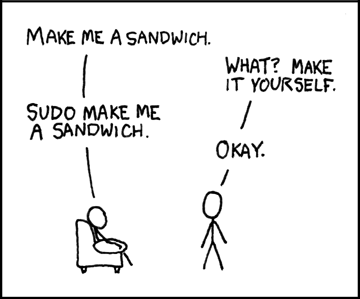
\includegraphics{images/sandwich.png}
\caption{Sudo sandwich from xkcd}
\end{figure}

Ok, so we now have RAxML installed. To run it, you could use the very handy \texttt{ips} package to call it from R, but it doesn't have an interface to all of the relevant commands. Instead, we're going to just create some commands to run ourselves.

First, we need sample data sets. We will be using ones, modified somewhat, from \href{http://sco.h-its.org/exelixis/web/software/raxml/hands_on.html}{this tutorial}. The original files are \href{http://sco.h-its.org/exelixis/resource/download/hands-on/Hands-On.tar.bz2}{here} but the modified ones are in the \href{https://github.com/PhyloMeth/LikelihoodTrees}{repository for this PhyloMeth exercise} in the \texttt{/inst/extdata} folder.

Until now, we've seen NEXUS files, which can include data blocks. RAxML uses Phylip-formatted files instead, which are simpler: a line that has the number of taxa and the number of sites, followed by one line per taxon with the taxon name, a space, and then the characters (though there could be interleaving).

\hypertarget{morphology-search}{%
\subsection{Morphology search}\label{morphology-search}}

First, we are going to examine morphology using likelihood. While morphology is typically analyzed with parsimony, there are models for morphology (i.e., Lewis 2001) and research suggests (Wright \& Hillis, 2014) that such models outperform parsimony for morphology, in addition to being less prone (in theory) to long branch attraction (Felsenstein 1978). Therefore, absent strongly held concerns rooted in an \href{http://onlinelibrary.wiley.com/doi/10.1111/cla.12148/full}{epistemological paradigm}, it seems prudent to use a parametric model for morphology (note this can be done in likelihood or Bayesian contexts).

Get the \href{https://github.com/PhyloMeth/LikelihoodTrees}{exercise} and \textbf{complete the \texttt{InferMorphologyTree\_exercise} function in \texttt{exercise.R}}. Also, look at the data in a text editor to get a sense of the structure. Which taxa are going to be lumped into clades, do you think? Some important things to note:

\begin{itemize}
\tightlist
\item
  Morphology (as well as some other data, such as SNPs) often includes only variable sites. This can cause a problem if not accounted for (it looks like all sites are evolving really fast, because the slow ones are ignored). There are corrections for this, three of which are implemented in RAxML.
\item
  RAxML creates a starting tree, then does a parsimony optimization, then likelihood. This is not a full parsimony search, though.
\item
  Remember that for nearly all tree searches, heuristic methods are used. That means that you are not guaranteed to get the best tree; given the size of tree space, one could almost say you're guaranteed not to find the best tree.
\item
  Computers are great at being logical. The downside is that they are terrible at being random. They often use the current time as a ``seed'' to get a pseudorandom number. You could think of it (this is more of an analogy than a description) as if the computer had a long table of stored ``random'' numbers, and that it started using numbers at the row corresponding to the number of seconds elapsed between the current time and some fixed date in the past. If you start two runs at different times, they'll have different numbers, but if you start them at the same time, they'll have the same ones. For tree search, there are often random moves: which branch is broken off and moved somewhere else. If you start two searches at the same time, thinking you're doing two independent searches, they'll perform exactly the same, despite the ``randomness''. RAxML asks users to supply a random number seed to it. If you use the same one across runs, they'll be exactly the same.
\end{itemize}

\hypertarget{dna}{%
\subsection{DNA}\label{dna}}

Most phylogenetic analyses for extant organisms use sequence data. This is often presented as DNA, though sometimes the data are translated to amino acids instead. Usually sequences from multiple genes are concatenated. There are a wide range of models available for sequence evolution. For DNA, the most popular remains general time reversible (GTR): a model that allows for a different transition rate between every pair of nucleotides, subject to the constraint that the rate from nucleotide \emph{i} to \emph{j} is the same as the rate from \emph{j} to \emph{i}. Different sites evolve at different rates (think of the sites coding for the active site of an enzyme versus those in an intron that has little to no functional purpose). One way to model this heterogeneity is with a gamma distribution: the likelihood is evaluated using several different rates for that site (Yang 1995). One can also apply partitions: allow different sections of the data to have different rates. This is commonly done to allow first, second, and third codon positions to have different rates, or to allow different genes to have different models of evolution. This can offer dramatic improvements in the fit of a model to the data; it is especially important when dealing with gappy data, such as cases where one gene is present for all taxa but another gene has ben sampled for only a subset of taxa.

\textbf{Do InferDNATreeWithBootstrappingAndPartitions\_exercise() in the homework}. Once this is done, install this homework library into R. From the folder containing the homework:

\begin{verbatim}
R CMD INSTALL LikelihoodTrees
\end{verbatim}

Then, in R:

\begin{verbatim}
library(PhyloMethLikelihoodTrees)
results <- InferDNATreeWithBootstrappingAndPartitions_exercise()
\end{verbatim}

Though you may have to include other arguments (especially \texttt{input.path}).

You can \textbf{plot your final tree}:

\begin{verbatim}
library(ape)
plot.phylo(results$ml.with.bs.tree, show.node.label=TRUE)
\end{verbatim}

This shows the branch lengths of the best ML tree and the bootstrap proportions. This is from a non-parametric bootstrap (Felsenstein 1985): the columns of data are sampled with replacement and then a tree search is redone. The more times a bipartition (an edge) on a tree is recovered, the more confidence we have in it (but this is not the same as the probability of it being true). Note one common error: the numbers reported, and in this case shown at nodes, are \emph{not} properties of a node or a clade: they are bipartitions: taxa A, C, E fall attach (perhaps through other nodes) to one end of an edge, and taxa B, D, E, F, G, H are attached to the other end.

\hypertarget{gene-tree-species-tree}{%
\section{Gene Tree Species Tree}\label{gene-tree-species-tree}}

\hypertarget{objectives-7}{%
\subsection{Objectives}\label{objectives-7}}

By the end of this chapter, you will:

\begin{itemize}
\tightlist
\item
  Understand why gene trees and species trees may not always agree
\item
  Know about some of the approaches in this area
\item
  Understand about phylogenetic networks
\end{itemize}

First, we will be looking at distinctions between gene trees and species trees. For this, we'll be using Liang Liu's phybase package. This isn't on CRAN, but it is available on his \href{https://faculty.franklin.uga.edu/lliu/content/phybase?}{website}. However, we'll be using a version I modified slightly and put on github. Liang's package uses \href{http://evolution.genetics.washington.edu/phylip/newicktree.html}{newick} format (yes, named after the \href{http://newicks.com}{restaurant}), but with additional options for including population size (branch width, included as a \texttt{\#} sign followed by a number) as well as the more traditional branch length. Both matter for coalescence: two copies are much more likely to have coalesced on a long, narrow branch than a short, fat one. Most packages in R instead use ape's \texttt{phylo} format, so I wrote a few functions to deal with that. This version of the package is on github; to install it:

\begin{verbatim}
library(devtools)
install_github("bomeara/phybase")
\end{verbatim}

For real science, Liang's is the canonical one (and definitely cite his) but this will be easier for us to use for class.

First, get a tree from Open Tree of Life. We'll get a recent plant tree from Beaulieu et al:

\begin{Shaded}
\begin{Highlighting}[]
\KeywordTok{library}\NormalTok{(rotl)}
\KeywordTok{library}\NormalTok{(ape)}
\NormalTok{phy <{-}}\StringTok{ }\KeywordTok{get\_study\_tree}\NormalTok{(}\StringTok{"ot\_485"}\NormalTok{, }\StringTok{"tree1"}\NormalTok{)}
\KeywordTok{plot}\NormalTok{(phy, }\DataTypeTok{cex=}\FloatTok{0.3}\NormalTok{)}
\end{Highlighting}
\end{Shaded}

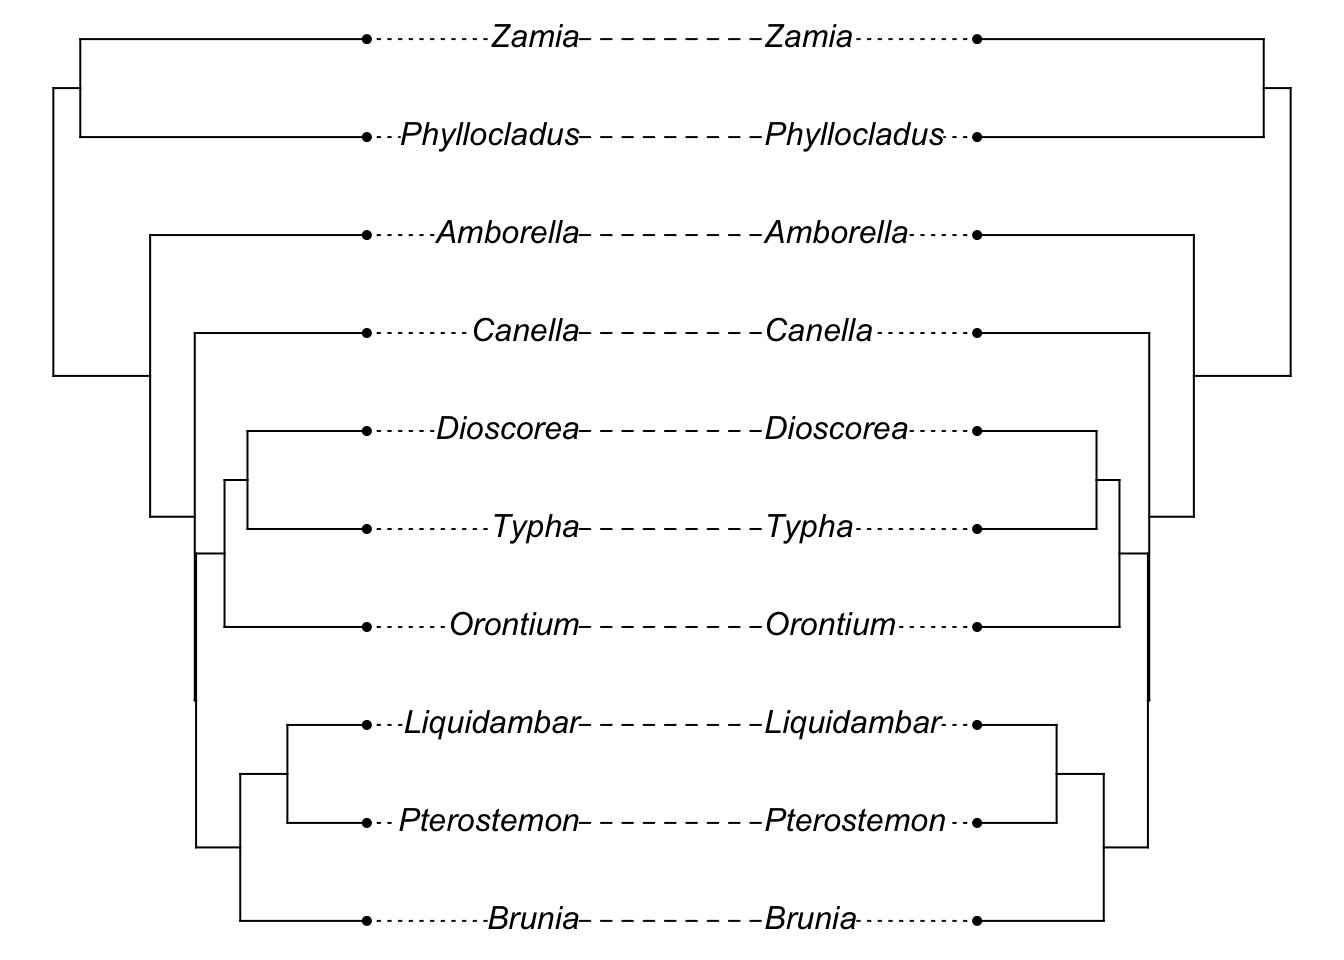
\includegraphics{comparative-methods_files/figure-latex/unnamed-chunk-19-1.pdf}

Let's simplify by dropping some taxa:

\begin{Shaded}
\begin{Highlighting}[]
\KeywordTok{library}\NormalTok{(geiger)}
\NormalTok{phy <{-}}\StringTok{ }\KeywordTok{drop.random}\NormalTok{(phy, }\KeywordTok{Ntip}\NormalTok{(phy) }\OperatorTok{{-}}\StringTok{ }\DecValTok{10}\NormalTok{)}
\KeywordTok{plot}\NormalTok{(phy)}
\KeywordTok{axisPhylo}\NormalTok{()}
\end{Highlighting}
\end{Shaded}

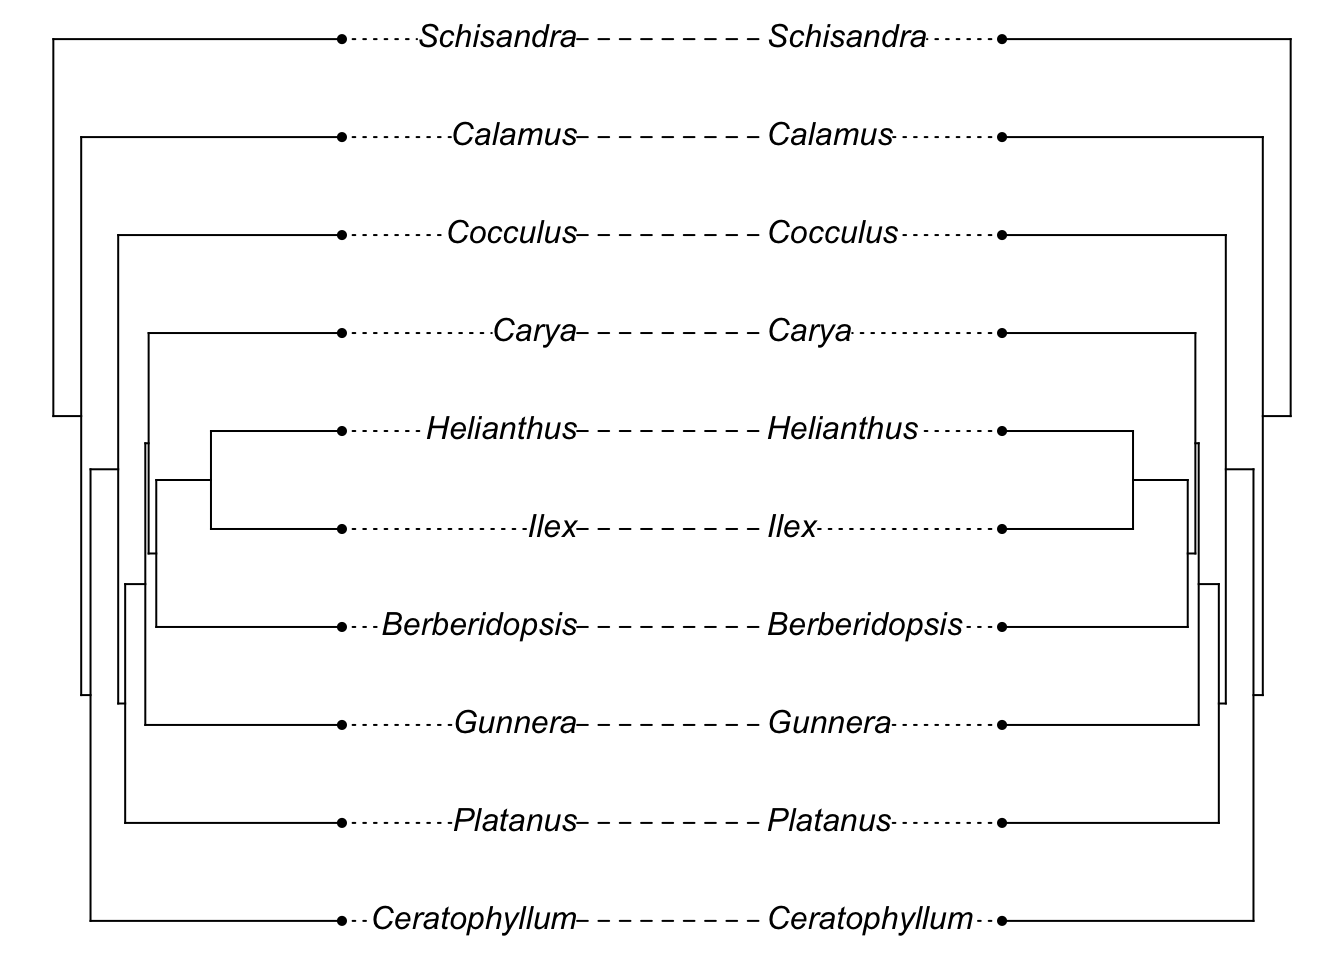
\includegraphics{comparative-methods_files/figure-latex/unnamed-chunk-20-1.pdf}

We can simulate gene trees on this tree:

\begin{Shaded}
\begin{Highlighting}[]
\KeywordTok{library}\NormalTok{(phybase)}
\NormalTok{gene.tree <{-}}\StringTok{ }\KeywordTok{sim.coaltree.phylo}\NormalTok{(phy, }\DataTypeTok{pop.size=}\FloatTok{1e{-}12}\NormalTok{)}
\KeywordTok{plot}\NormalTok{(gene.tree)}
\end{Highlighting}
\end{Shaded}

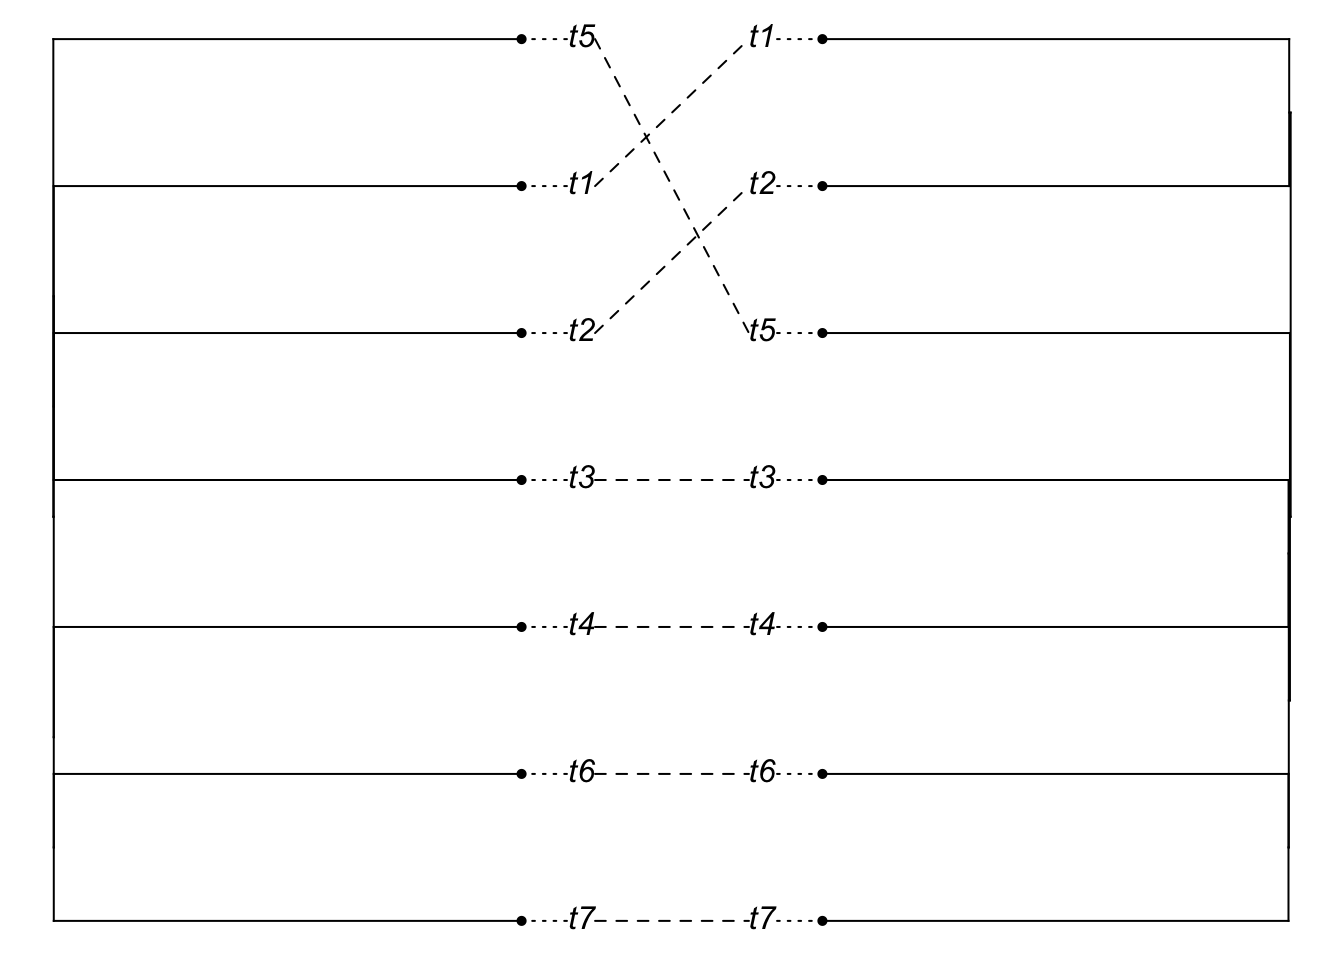
\includegraphics{comparative-methods_files/figure-latex/unnamed-chunk-21-1.pdf}

And it probably looks very similar to the initial tree:

\begin{Shaded}
\begin{Highlighting}[]
\KeywordTok{library}\NormalTok{(phytools)}
\KeywordTok{plot}\NormalTok{(}\KeywordTok{cophylo}\NormalTok{(phy, gene.tree, }\KeywordTok{cbind}\NormalTok{(}\KeywordTok{sort}\NormalTok{(phy}\OperatorTok{$}\NormalTok{tip.label), }\KeywordTok{sort}\NormalTok{(gene.tree}\OperatorTok{$}\NormalTok{tip.label))))}
\end{Highlighting}
\end{Shaded}

\begin{verbatim}
## Rotating nodes to optimize matching...
## Done.
\end{verbatim}

\includegraphics{comparative-methods_files/figure-latex/unnamed-chunk-22-1.pdf}

{[}Note I'm being a bit sloppy here: the initial branch lengths of the tree we used are in millions of years (i.e., 5 = 5 MY) while the coalescent sim is treating these as coalescent time units: there would be even lower chance of incongruence if we converted the former into the latter. Unfortunately, the simulator fails with branch lengths that are realistically long for this tree.{]}

So, does this mean gene tree species tree issues aren't a problem?

Well, it depends on the details of the tree. One common misconception is that gene tree species tree issues only relate to trees for recent events. This problem can happen any time there are short, fat branches, where lack of coalescence of copies can occur.

\begin{Shaded}
\begin{Highlighting}[]
\NormalTok{species.tree <{-}}\StringTok{ }\KeywordTok{rcoal}\NormalTok{(}\DecValTok{7}\NormalTok{)}
\NormalTok{species.tree}\OperatorTok{$}\NormalTok{edge.length <{-}}\StringTok{ }\NormalTok{species.tree}\OperatorTok{$}\NormalTok{edge.length }\OperatorTok{/}\StringTok{ }\NormalTok{(}\DecValTok{10}\OperatorTok{*}\KeywordTok{max}\NormalTok{(}\KeywordTok{branching.times}\NormalTok{(species.tree)))}
\NormalTok{gene.tree <{-}}\StringTok{ }\KeywordTok{sim.coaltree.phylo}\NormalTok{(species.tree)}
\KeywordTok{plot}\NormalTok{(}\KeywordTok{cophylo}\NormalTok{(species.tree, gene.tree, }\KeywordTok{cbind}\NormalTok{(}\KeywordTok{sort}\NormalTok{(species.tree}\OperatorTok{$}\NormalTok{tip.label), }\KeywordTok{sort}\NormalTok{(gene.tree}\OperatorTok{$}\NormalTok{tip.label))))}
\end{Highlighting}
\end{Shaded}

\begin{verbatim}
## Rotating nodes to optimize matching...
## Done.
\end{verbatim}

\includegraphics{comparative-methods_files/figure-latex/unnamed-chunk-23-1.pdf}

You should see (in most iterations), the above code giving a mismatch between the gene tree and the species tree (the species tree has little height). Now, let's lengthen the tips of the species tree:

\begin{Shaded}
\begin{Highlighting}[]
\NormalTok{tip.rows <{-}}\StringTok{ }\KeywordTok{which}\NormalTok{(species.tree}\OperatorTok{$}\NormalTok{edge[,}\DecValTok{2}\NormalTok{]}\OperatorTok{<=}\KeywordTok{Ntip}\NormalTok{(species.tree))}
\NormalTok{species.tree2 <{-}}\StringTok{ }\NormalTok{species.tree}
\NormalTok{species.tree2}\OperatorTok{$}\NormalTok{edge.length[tip.rows] <{-}}\StringTok{ }\DecValTok{100} \OperatorTok{+}\StringTok{ }\NormalTok{species.tree2}\OperatorTok{$}\NormalTok{edge.length[tip.rows]}
\NormalTok{gene.tree2 <{-}}\StringTok{ }\KeywordTok{sim.coaltree.phylo}\NormalTok{(species.tree2)}
\KeywordTok{plot}\NormalTok{(}\KeywordTok{cophylo}\NormalTok{(species.tree2, gene.tree2, }\KeywordTok{cbind}\NormalTok{(}\KeywordTok{sort}\NormalTok{(species.tree2}\OperatorTok{$}\NormalTok{tip.label), }\KeywordTok{sort}\NormalTok{(gene.tree2}\OperatorTok{$}\NormalTok{tip.label))))}
\end{Highlighting}
\end{Shaded}

\begin{verbatim}
## Rotating nodes to optimize matching...
## Done.
\end{verbatim}

\includegraphics{comparative-methods_files/figure-latex/unnamed-chunk-24-1.pdf}

It looks like a mismatch, but it's hard to see, since the tips are so long. So plot the cladogram instead {[}we need to manually change branch lengths to do this, though note we do not resimulate the gene tree{]}.

\begin{Shaded}
\begin{Highlighting}[]
\NormalTok{species.tree2.clado <{-}}\StringTok{ }\KeywordTok{compute.brlen}\NormalTok{(species.tree2)}
\NormalTok{gene.tree2.clado <{-}}\StringTok{ }\KeywordTok{compute.brlen}\NormalTok{(gene.tree2)}
\KeywordTok{plot}\NormalTok{(}\KeywordTok{cophylo}\NormalTok{(species.tree2.clado, gene.tree2.clado, }\KeywordTok{cbind}\NormalTok{(}\KeywordTok{sort}\NormalTok{(species.tree2.clado}\OperatorTok{$}\NormalTok{tip.label),}
\KeywordTok{sort}\NormalTok{(gene.tree2.clado}\OperatorTok{$}\NormalTok{tip.label))))}
\end{Highlighting}
\end{Shaded}

\begin{verbatim}
## Rotating nodes to optimize matching...
## Done.
\end{verbatim}

\includegraphics{comparative-methods_files/figure-latex/unnamed-chunk-25-1.pdf}

So we can see that even though the relevant divergences happened long ago, gene tree species tree issues are still a problem.

\hypertarget{dating}{%
\section{Dating}\label{dating}}

\hypertarget{objectives-8}{%
\subsection{Objectives}\label{objectives-8}}

By the end of this chapter, you will:

\begin{itemize}
\tightlist
\item
  Understand dating algorithms
\item
  Be able to use r8s and BEAST
\item
  Be afraid of calibrations
\end{itemize}

Make sure to \textbf{read the relevant papers}: \url{https://www.mendeley.com/groups/8111971/phylometh/papers/added/0/tag/week5/}

To do this week's assignments, you will have to:

\begin{itemize}
\tightlist
\item
  \textbf{Download and install r8s} from \url{http://ceiba.biosci.arizona.edu/r8s/index.html}
\item
  \textbf{Download BEAST2 and Beauti} (come together), \textbf{TreeAnnotator}, and \textbf{Tracer} from \url{http://beast2.org} and \url{http://beast.bio.ed.ac.uk/tracer}.
\item
  \textbf{Install a tweaked version of Geiger}

  \begin{itemize}
  \tightlist
  \item
    \texttt{library(devtools)}
  \item
    \texttt{install\_github("bomeara/geiger-v2")} (eventually I'll make a pull request)
  \end{itemize}
\end{itemize}

\hypertarget{beast}{%
\subsection{BEAST}\label{beast}}

For the BEAST part, we're not going to do our testing via R package approach: dealing with file paths and such are too problematic. So we'll just go through an exercise, but unlike many canned tutorials, you'll have to figure out what to do at stages. Note that this is based on the \href{https://github.com/CompEvol/beast2/blob/master/doc/tutorials/DivergenceDating/DivergenceDatingTutorialv2.0.3.pdf?raw=true}{tutorial} by Drummond, Rambaut, and Bouckaert. A tutorial that provides far more background info and other context than anything on the Beast2 website is Tracy Heath's \href{http://phyloworks.org/workshops/DivTime_BEAST2_tutorial_FBD.pdf}{tutorial} from the Bodega Bay Workshop in Applied Phylogenetics: if you are going to run BEAST, read that. There is also now a \href{http://beast2.org/book/}{book} that you can buy.

BEAST uses XML files for commands, rather than NEXUS files (though it does use NEXUS files for data). This XML format is different from \href{http://www.nexml.org}{NeXML} and \href{http://www.phyloxml.org}{PhyloXML}, two other XML formats proposed for phylogenetics (though, as of now, they're still not used much in the field -- most students won't encounter them). These files are often made using the program BEAUTi (also from the BEAST developers) and then, sometimes, hand edited.

\begin{enumerate}
\def\labelenumi{\arabic{enumi}.}
\tightlist
\item
  \textbf{Import primates-mtDNA.nex} into BEAUTi; it's includided in examples/nexus in the BEAST folder. Note it's File -\textgreater{} Import alignment.
\item
  But wait -- what are you loading? Have you looked at the file? Open it in a text editor (or R, or Mesquite) and look at it. Do you believe the sequences are aligned properly? Is there anything weird about them? This is an essential step.
\item
  We will be partitioning, as with RAxML. This file already has some partitions, but some overlap (coding vs the three codon positions). Delete the coding partition using the \texttt{-} sign button on the bottom of the window.
\item
  Partitions can be linked: allow different rates but the same topology, for example. Select all four partitions and click Link Trees. Then click on the first pull down (for noncoding) for the Tree column and name it ``tree''. Do the same for Clock (rename to ``clock'').
\item
  Temporarily link sites in the same way.
\item
  BEAST has a variety of models. We're going to do HKY (so, two different rates) with gamma-distributed rate differences. To do this:

  \begin{itemize}
  \tightlist
  \item
    Set Gamma Category Count to 4
  \item
    Set the Shape to be estimated
  \item
    Select the HKY model
  \item
    Make sure Kappa is estimated
  \item
    Make sure frequences are estimated
  \item
    Select estimate for Substitution Rate
  \end{itemize}
\item
  Go back to partitions and click on Unlink Site Models. This lets each partition have its own HKY+gamma model (and doing the link -\textgreater{} set -\textgreater{} unlink lets you save on work of setting it for each one).
\item
  We need to choose a clock model. A Strict Clock is the classic molecular clock. Most people using BEAST (and this is based on various sim studies) use relaxed clock log normal, so choose that. Having the number of discrete rates set to -1 will allow as many rates as branches.
\item
  Now comes the tricky bit: setting your priors. For example, you need a prior for the tree: assume a Yule prior (only speciation events, no extinction)? Or a birth-death one? {[}and think about the implications of these choices for later analyses -- estimating extinction rates, for example{]}. And even if you have a belief about whether extinction might have happened or not, what about parameters like gamma shape for first codon position sites? Exponential, beta, etc.? You probably don't have a good idea of what they should be in terms of shape, let alone priors for the actual values. And this might affect your analyses: the result is due to the prior and the likelihood. Let's leave all the priors set to the default for now, except for the tree: do a birth-death model for that.
\item
  We can also add priors: say, a prior for the age of a node.

  \begin{itemize}
  \tightlist
  \item
    Click on the ``+'' button
  \item
    Call the Taxon set label ``human-chimp''
  \item
    Click on Homo\_sapiens and then the ``\textgreater\textgreater{}'' button
  \item
    Do the same for Pan
  \item
    Click ok
  \item
    Force it to be monophyletic
  \item
    Choose Log Normal for the age prior
  \item
    Select mean in real space (so it's easier for us to understand the age)
  \item
    Enter 6 (for 6 MY) for the M = mean of the distribution
  \item
    \textbf{Select a value for S that leads to a 95\% range of about 5-7 MY (use the information on the right side of the window to help)}
  \end{itemize}
\item
  Go to MCMC to set parameters for the run

  \begin{itemize}
  \tightlist
  \item
    Do 1M generations to start
  \item
    You can also set how often the info is saved to disk or printed on the screen. Change the tracelog to primates\_birthdeath\_prior.log
  \end{itemize}
\item
  Save this in the same folder as your original nexus file: maybe store as primates\_birthdeath\_prior.xml.
\item
  Yay! We have created a file with commands to run BEAST. Open it in a text editor and look at it (don't modify or save it).
\item
  Now open BEAST. Choose the xml file you just made and run.
\item
  Time passes.
\item
  Now open the log file in Tracer. Investigate some of the statistics, including looking at ESS: effective sample size. Ones that aren't black indicate ones that did not run long enough.
\item
  Go back to BEAUTi.

  \begin{itemize}
  \tightlist
  \item
    Change the tree prior to a Yule tree
  \item
    Change the tracelog to primates\_yule\_prior.log and change the tree file name
  \item
    Save as the file to primates\_yule\_prior.xml
  \end{itemize}
\item
  Use this new xml file to run BEAST again.
\item
  Now look at this log file with the other one, both in Tracer. Are the estimates the same? Even for something like tree height? What does this suggest?
\item
  Use TreeAnnotator on one of your tree files to summarize.

  \begin{itemize}
  \tightlist
  \item
    Decide what the burnin should be: that is the number of trees (not number of generations) to delete.
  \item
    Change Posterior probability limit to 0: if you are going to show an edge, you should show the support for that. Many people only show support above 50\% but still show all branches: this is problematic (only showing uncertainty on the edges where uncertainty is relatively low).
  \end{itemize}
\item
  FigTree or R can be used to visualize the final tree with support.
\end{enumerate}

\#\#r8s

r8s implements several functions for converting a phylogram to a chronogram. It does the classic, Langley-Fitch molecular clock which stretches branches but assumes a constant rate for all. It also implements two algorithms by Sanderson: nonparametric rate smoothing (NPRS) and penalized likelihood (PL). Both relax the assumption of constant rate of evolution and instead allow rates to vary along the tree. NPRS tries to minimize rate changes at nodes. PL has a model for changes (to give likelihood of original branch lengths) and combines this with a nonparametric penalty for rate changes. It tries to minimize the combination of these two parameters, but there is a user-set penalty to decide the relative value of these in the combined sum. This is set by cross-validation: delete some data, estimate parameters, predict the deleted data, and see how close the deleted data are to the simulated data. In this case, the datum deleted is a single tip, and the length of this branch is the value to predict. This can now happen within r8s. In general, PL is more accurate than NPRS, but is slower (but both are much faster than BEAST). \texttt{treepl} is a later program that implements Sanderson's algorithms but can work on much larger trees.

Jon Eastman coded an interface to this in Geiger, but it wasn't exposed to users. I've added some additional features (including an \texttt{ez.run} mode) and documentation to his code. This is now in a fork of Geiger, but I'll file a pull request soon to put it into the main code. For now, make sure you have installed the forked version:

\begin{verbatim}
devtools::install_github("bomeara/geiger-v2")
library(geiger)
\end{verbatim}

Then use the help for \texttt{?r8s.phylo} to figure out how to use this function. Also look at the \href{http://loco.biosci.arizona.edu/r8s/r8s1.7.manual.pdf}{r8s manual} to understand the options.

\textbf{Run the examples} in Geiger for this. You can also look at the examples that come with r8s.

\hypertarget{applying-to-your-own-work}{%
\subsection{Applying to your own work}\label{applying-to-your-own-work}}

By this point in the course, you should be thirsting to apply these tools to your own questions. Do so! \textbf{Get a dataset (think back to the getting trees method), infer a tree (if needed), and date it using one of these approaches.} I'd advise making your own github repository for this. You could pay to keep it secret; I'd advise it's probably not worth it (there is some risk of being scooped, but it's pretty low) but it's your call.

\hypertarget{visualizing-trees-and-trees-with-data}{%
\section{Visualizing trees and trees with data}\label{visualizing-trees-and-trees-with-data}}

\hypertarget{objectives-9}{%
\subsection{Objectives}\label{objectives-9}}

By the end of this chapter, you will:

\begin{itemize}
\tightlist
\item
  Understand ways to visualize trees
\item
  Understand how to visualize trees with data
\end{itemize}

It's always important to visualize trees, and data on your trees. For example, most comparative methods require branch lengths. Are yours reasonable? Do you have any taxa on very long branches (which could indicate alignment or paralogy issues)? Are there many effectively zero length branches? Does everything agree with what you know of taxonomy?

To start, let's take a sample tree: a tree of snakes by Pyron R.A., Burbrink F., Colli G., Montes de oca A.N., Vitt L.J., Kuczynski C.A., \& Wiens J.J. 2010. The phylogeny of advanced snakes (Colubroidea), with discovery of a new subfamily and comparison of support methods for likelihood trees. Molecular Phylogenetics and Evolution 58 (2): 329-342. {[}\#TODO: add proper citation{]}. It is a tree of 767 taxa. But we'll start with a 12 tip subtree.

The natural way you'd plot this in R:

\begin{Shaded}
\begin{Highlighting}[]
\NormalTok{ape}\OperatorTok{::}\KeywordTok{plot.phylo}\NormalTok{(small.phy)}
\end{Highlighting}
\end{Shaded}

\includegraphics{comparative-methods_files/figure-latex/unnamed-chunk-28-1.pdf}

Plotting it with tips to the right is most common, but there are other options, too:

\begin{Shaded}
\begin{Highlighting}[]
\NormalTok{ape}\OperatorTok{::}\KeywordTok{plot.phylo}\NormalTok{(small.phy, }\DataTypeTok{direction=}\StringTok{"upwards"}\NormalTok{)}
\end{Highlighting}
\end{Shaded}

\includegraphics{comparative-methods_files/figure-latex/unnamed-chunk-29-1.pdf}

Especially for big trees, fan (circle trees) can also be popular:

\begin{Shaded}
\begin{Highlighting}[]
\NormalTok{ape}\OperatorTok{::}\KeywordTok{plot.phylo}\NormalTok{(small.phy, }\DataTypeTok{type=}\StringTok{"fan"}\NormalTok{)}
\end{Highlighting}
\end{Shaded}

\includegraphics{comparative-methods_files/figure-latex/unnamed-chunk-30-1.pdf}
Sometimes for just seeing the tree structure itself, once can remove branch lengths:

\begin{Shaded}
\begin{Highlighting}[]
\NormalTok{ape}\OperatorTok{::}\KeywordTok{plot.phylo}\NormalTok{(small.phy, }\DataTypeTok{type=}\StringTok{"cladogram"}\NormalTok{)}
\end{Highlighting}
\end{Shaded}

\includegraphics{comparative-methods_files/figure-latex/unnamed-chunk-31-1.pdf}

  \bibliography{packages.bib,zotero.bib}

\end{document}
